\documentclass{beamer}
\usepackage[utf8]{inputenc}
\usepackage[portuguese]{babel}
\usepackage{amsmath}
\usepackage{subfigure}
\usepackage{booktabs}

\usetheme{metropolis}           % Use metropolis theme

\newtheorem{mydefinition}{Definição}

\newcommand{\foreignword}[1]{\textit{#1}}
\newcommand{\toolname}[1]{\textit{#1}}
\newcommand{\fieldR}{\mathbb{R}}
\newcommand{\powerset}{\mathcal{P}}
\newcommand{\probability}{\mathbb{P}}
\newcommand{\expectation}{\mathbb{E}}
\newcommand{\algname}[1]{\texttt{#1}}
\newcommand{\langname}[1]{\texttt{#1}}
\newcommand{\varname}[1]{\texttt{#1}}
\newcommand{\floor}[1]{\lfloor #1 \rfloor}
\newcommand{\ceil}[1]{\lceil #1 \rceil}
\newcommand{\mathsc}[1]{{\normalfont\textsc{#1}}}
\newcommand{\forest}{\mathcal{F}}
\newcommand{\pfsnode}[1]{\mathbf #1}
\newcommand{\species}[1]{\textit{#1}}
\newcommand{\gender}[1]{\textit{#1}}

\graphicspath{ {img/} }

\title{Projeto de Algoritmos Baseados em Florestas de Posets para o
Problema de Otimização U-curve}
\date{Novembro de 2017}
\author{Gustavo Estrela}
\institute{Instituto de Matemática e Estatística \\ 
           Centro de Toxinas, Resposta-imune e Sinalização Celular (CeTICS) \\
           Laboratório Especial de Ciclo Celular, Instituto Butantan}
\begin{document}
  \maketitle
    
  \section{O problema U-curve}

\begin{frame}{Modelos computacionais}
  Modelos computacionais são criados para simular sistemas complexos. \\
  \pause
  \begin{center}
  %\alert{ 
  $
  \begin{aligned}
    \text{entrada} &\longrightarrow& \text{sistema} &\longrightarrow& \text{saída} \\
    \pause
    \text{entrada} &\longrightarrow& \text{modelo} &\longrightarrow& \sim\text{saída} \\
  \end{aligned}
  $
  %}
  \end{center}
\end{frame} 

\begin{frame}{Exemplo de modelo computacional}
  \begin{figure}
    \centering
    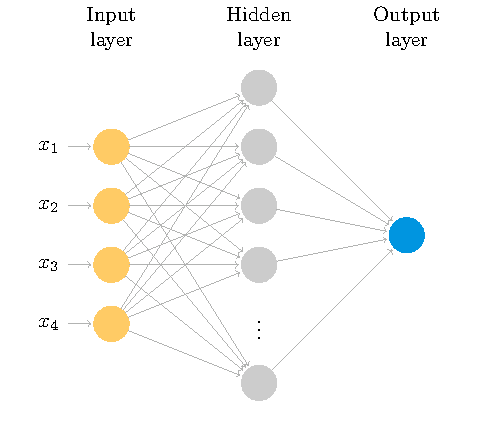
\includegraphics[clip=true]{neuralnet/neuralnet.pdf}
  \end{figure}
\end{frame}

\begin{frame}{O problema de seleção de características}
  A seleção de características é uma etapa da seleção de modelos. Ela
  deve escolher quais são as melhores características para se considerar
  no modelo.
  \pause
  \begin{mydefinition}
    Dado um conjunto $S$ de características e uma função 
    de custo $c$, ache o subconjunto de 
    $X \in \powerset(S)$ tal que $c (X)$ é mínimo.
  \end{mydefinition}
\end{frame}


\begin{frame}{O problema de seleção de características}
  Podemos representar um conjunto $X$ de características por um vetor
  de bits que chamamos de \alert{vetor característico}. \\
  %\pause
  %Assuma que o conjunto $S$ tem uma ordem $S = \langle s_1, s_2, ..., s_n \rangle$.
  %Então, se o conjunto $X$ possui a i-ésima característica de $S$, então
  %o i-ésimo bit do vetor característico deve estar ligado.
  \pause
  \vspace{1em}
  Por exemplo, se $S = \{s_1, s_2, s_3\}$ e $X = \{s_1, s_3\}$
  então o vetor característico de $X$ é $101$.
\end{frame}

\begin{frame}{O espaço de busca}
  Os algoritmos estudados neste trabalho representam o espaço de busca
  com o reticulado Booleano $(\powerset(S), \subseteq)$.
  \begin{figure}
    \centering
    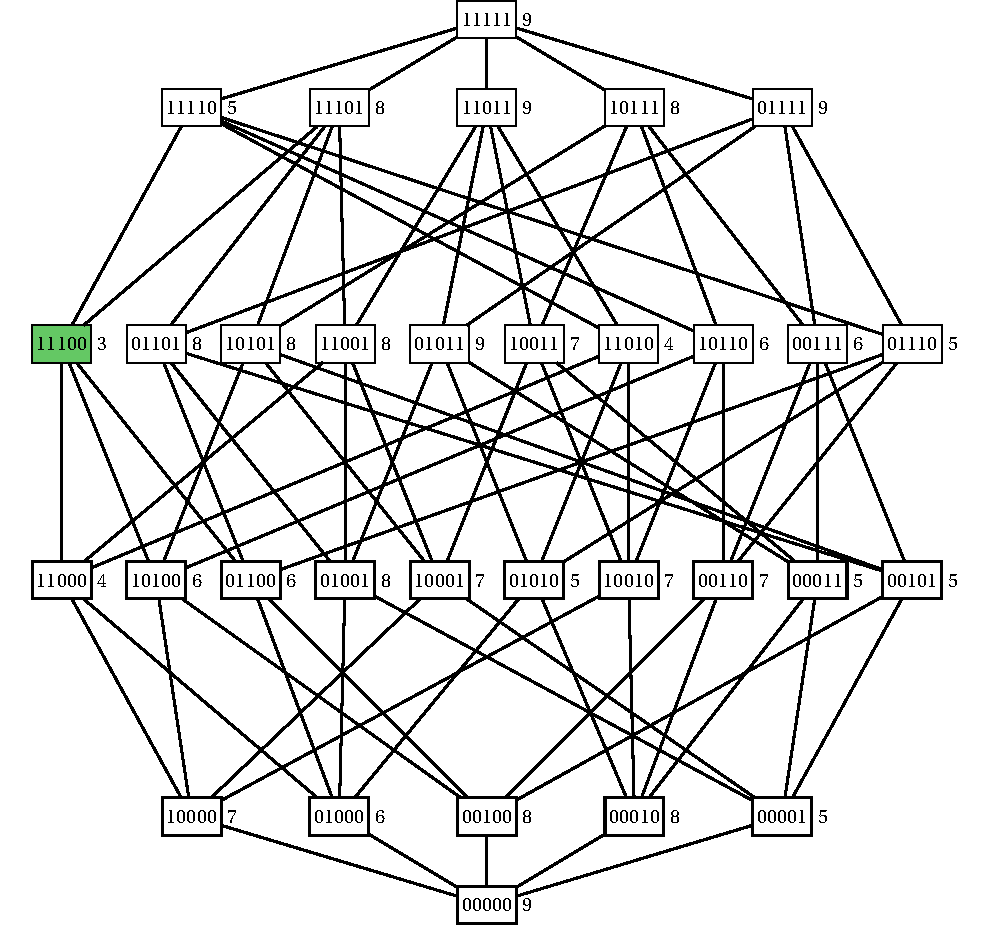
\includegraphics[clip=true, width=.6\textwidth]{lattice/Boolean_lattice.pdf}
  \end{figure}
\end{frame}

\begin{frame}{O espaço de busca}
  Chamamos de \alert{cadeia} uma sequência de conjuntos adjacentes 
  $X_1, X_2, \dots, X_n$ tal que $X_1 \subseteq X_2 \subseteq \dots \subseteq X_n$. 
  \pause
  \begin{figure}
    \centering
    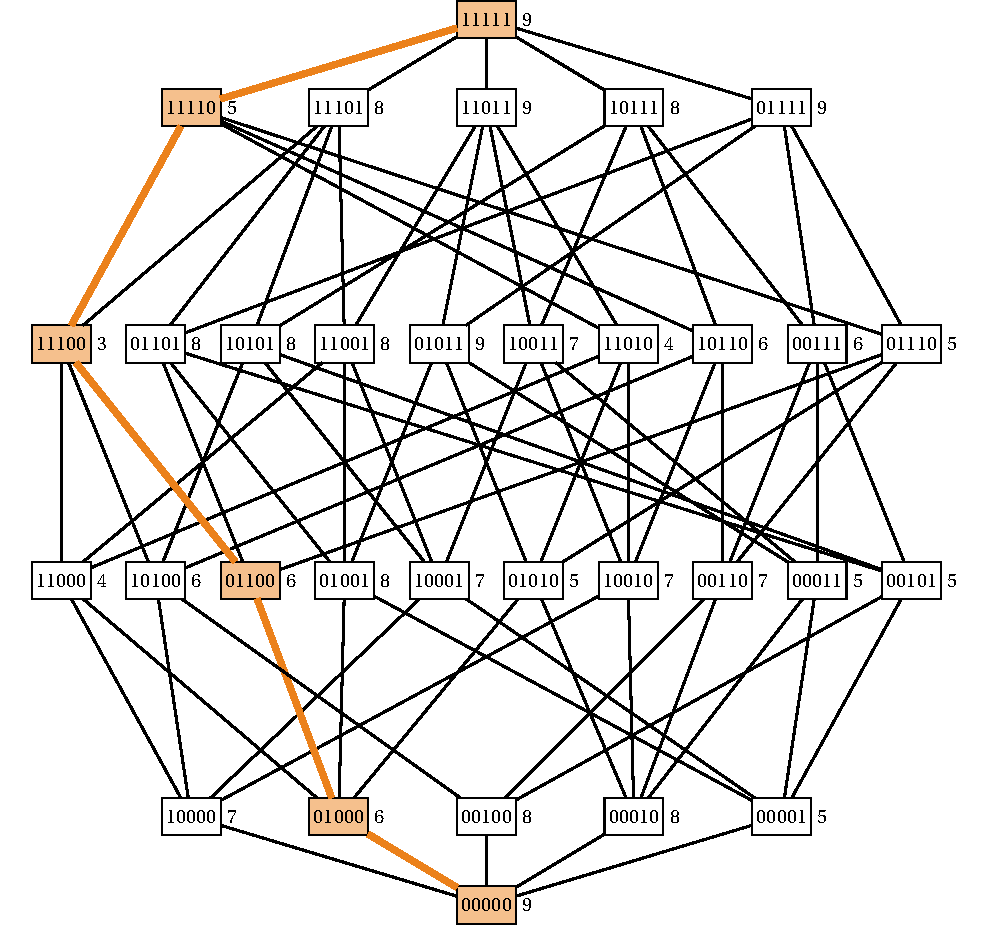
\includegraphics[clip=true, width=.6\textwidth]{lattice/chain.pdf}
  \end{figure}
\end{frame}

\begin{frame}{A função de custo}
  A função de custo $c$ deve refletir a qualidade de um conjunto de 
  características $X$ a ser usado no modelo.\\
  \pause
  \vspace{1em}
  Nestas funções, um fenômeno conhecido em aprendizado de máquina aparece.
  A função descreve curvas em U nas cadeias do reticulado.
  \begin{figure}[ht]
    \centering
    \begin{tabular}{c c}
    \subfigure {\scalebox{.4}{
        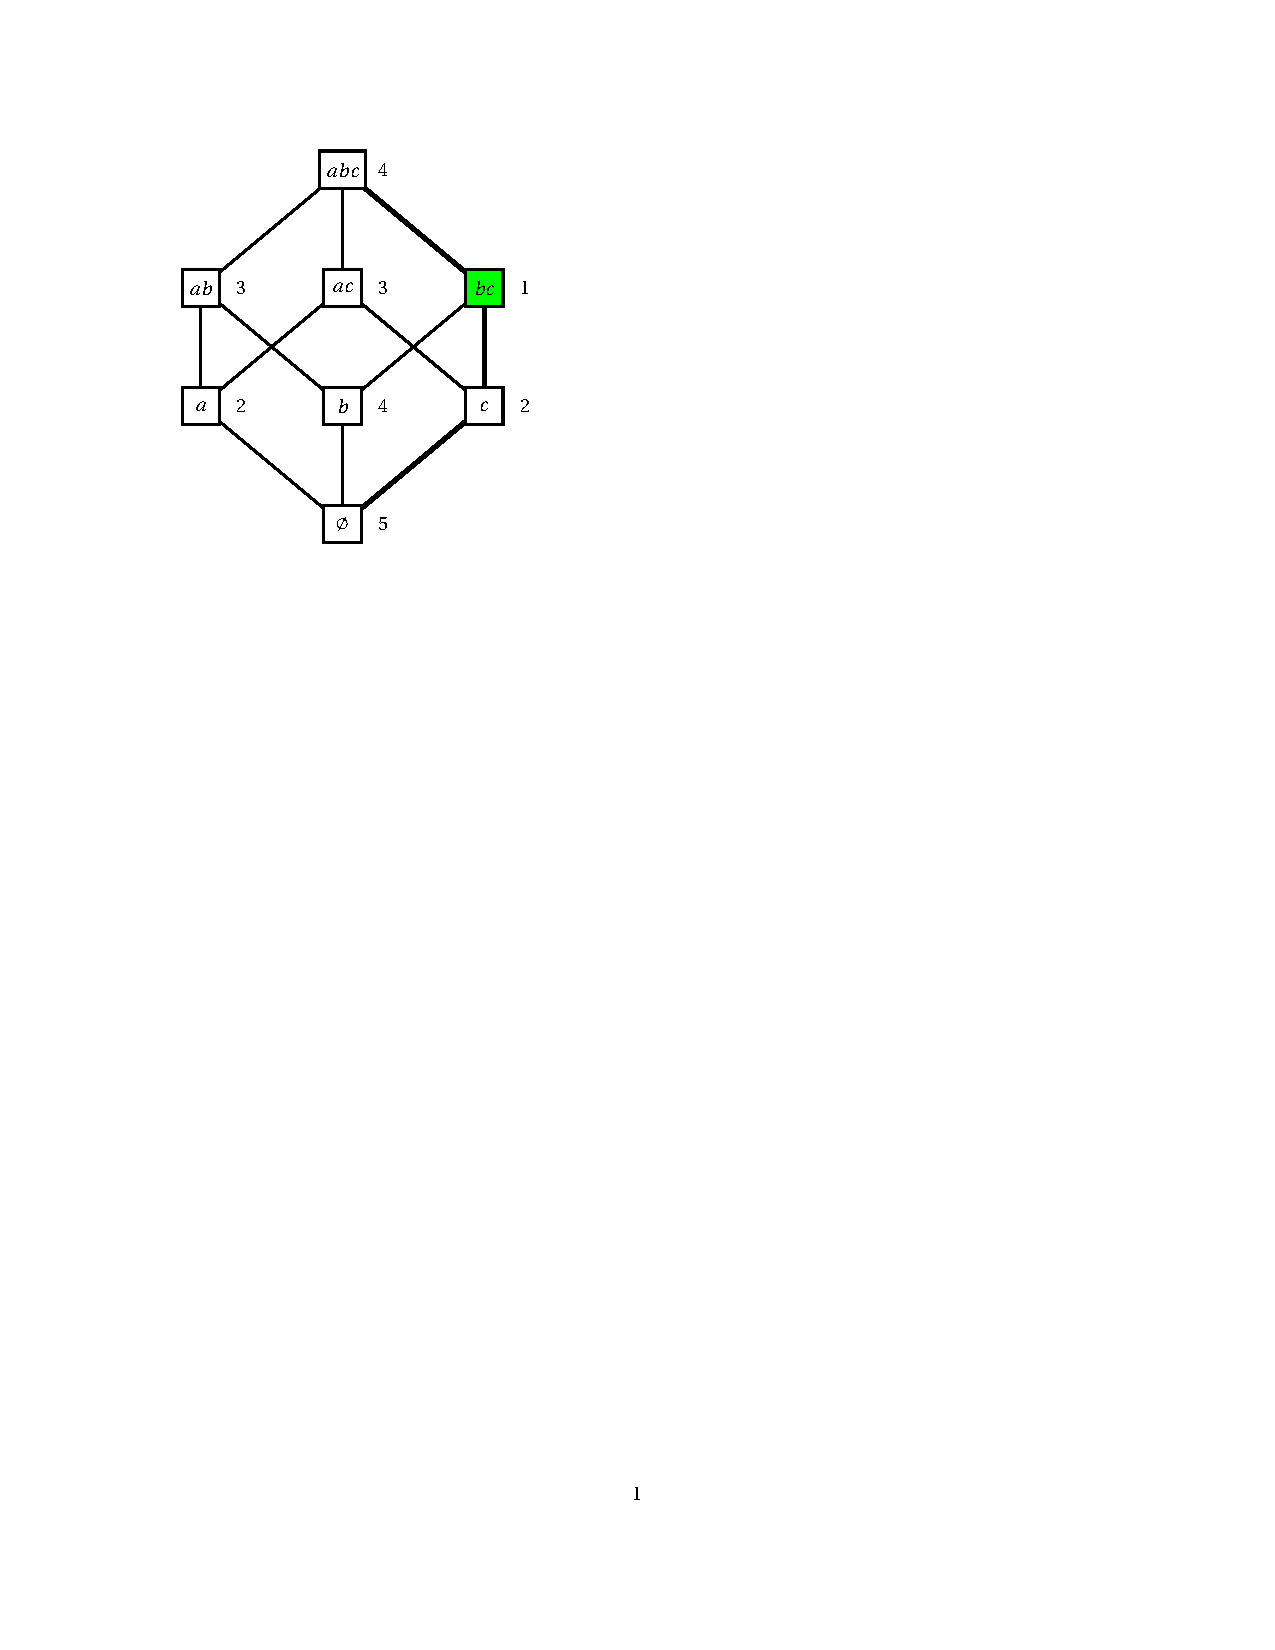
\includegraphics[clip=true, trim={3cm 18cm 13cm 2cm}]{intro/example_lattice_3.pdf}}
    \label{fig:intro:lattice} }
    & 
    \subfigure {\scalebox{.15}{
        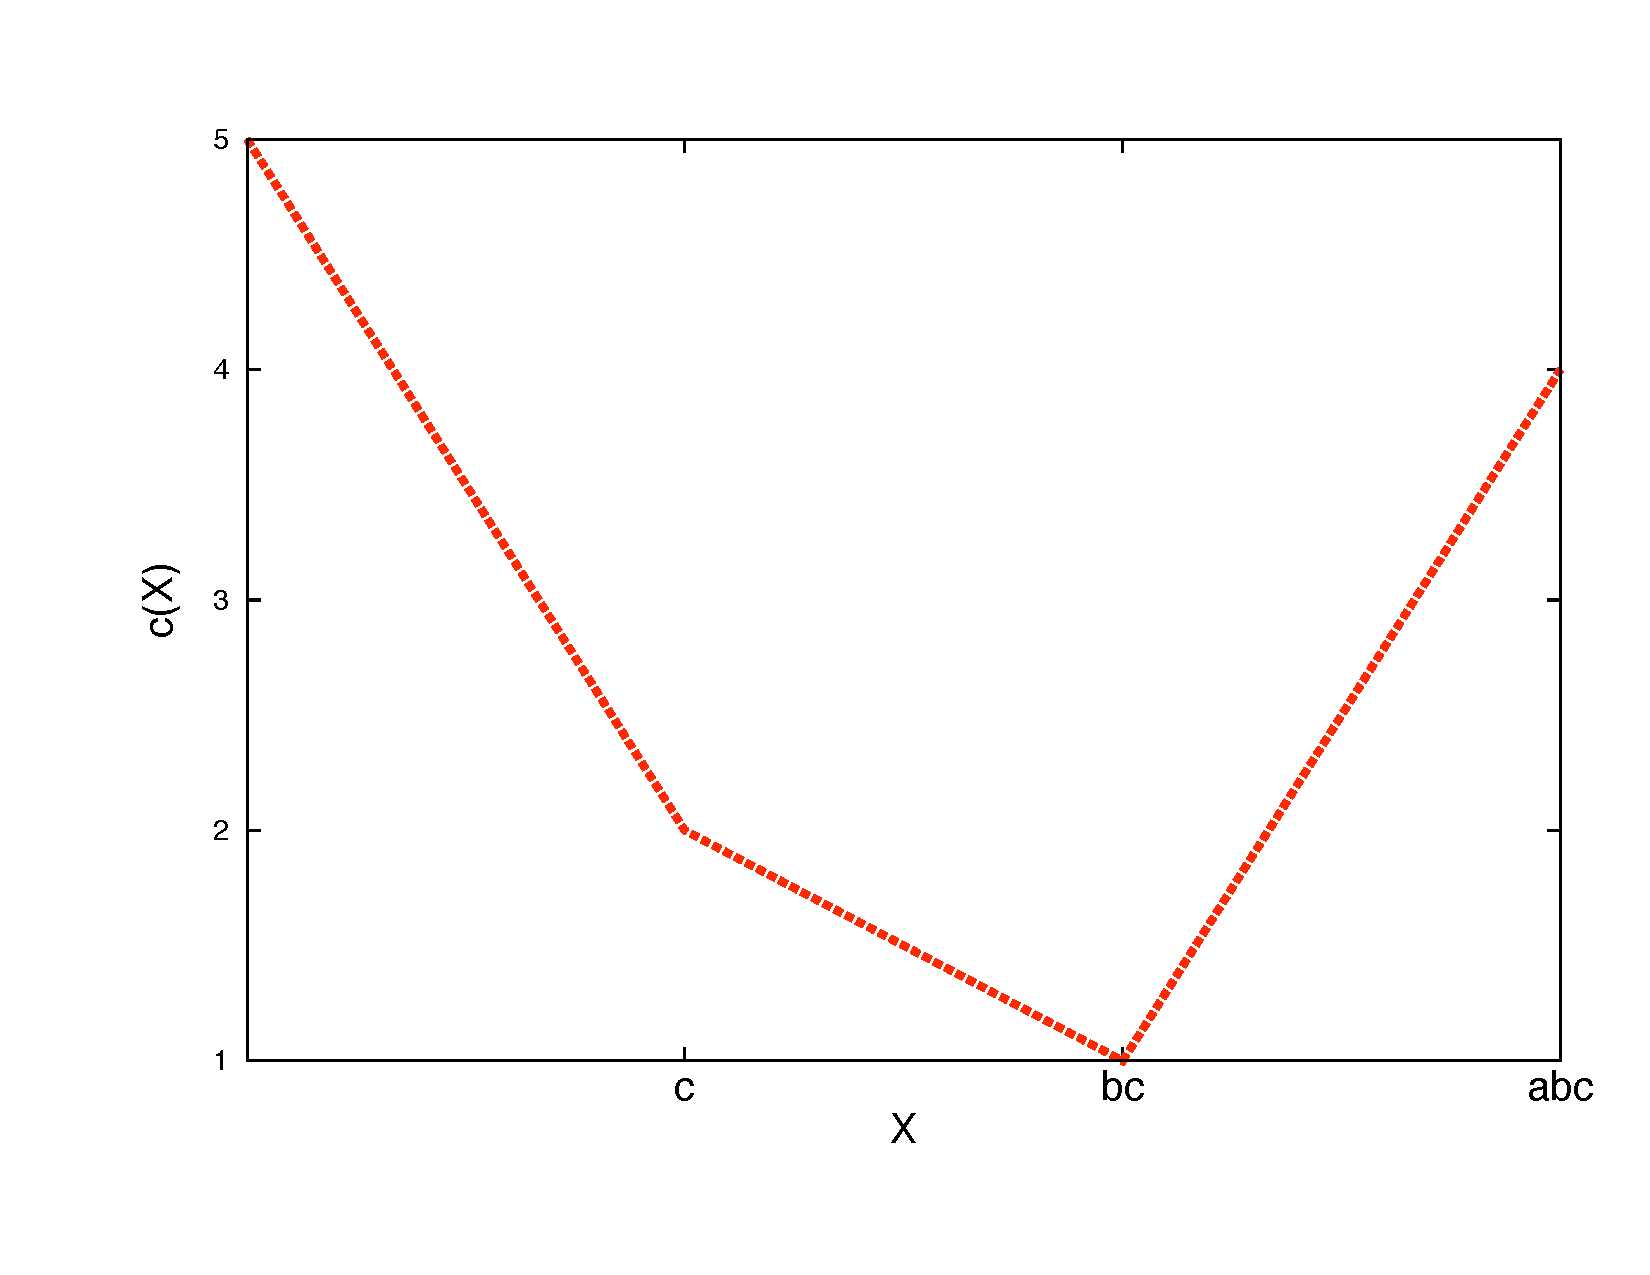
\includegraphics[clip=true, trim={1cm 0cm 1cm 2cm}]{intro/example_lattice_chain_3.pdf}}
    \label{fig:intro:chain} }
    \end{tabular}
\end{figure}
\end{frame}

\begin{frame}{Funções decomponíveis em curvas U}
\begin{mydefinition}\label{fund_concepts:ushape}
Uma função de custo $c$ é dita {\bf \em decomponível em curvas U} se
para toda cadeia maximal $X_1, ..., X_l$, $c(X_j) \leq max \{c (X_i),
c (X_k)\}$ sempre que $X_i \subseteq X_j \subseteq X_k$, $i, j, k \in 
\{1, ..., l\}$.
\end{mydefinition}
\end{frame}


\begin{frame}{O problema U-curve}
\begin{mydefinition}[Problema U-Curve]
Dados um conjunto finito e não-vazio $S$ e uma função de custo $c$ 
decomponível em curvas U, encontrar um subconjunto $X \in \powerset (S)$ 
tal que $c(X)$ é mínimo.
\end{mydefinition}
\end{frame}

\section{Algoritmos baseados em florestas}
\begin{frame}{O algoritmo \algname{U-Curve-Branch-and-Bound}}
O algoritmo \algname{U-Curve-Branch-and-Bound} (\algname{UBB}) organiza
o espaço de busca em uma árvore.
\begin{figure}[!ht]
  \centering 
  \begin{tabular}{c c}
    \subfigure {\scalebox{0.3}{
     \includegraphics[clip=true]{pfs/ubb/full_lattice.pdf}}
     \label{fig:ubb:full} }
    & 
    \subfigure {\scalebox{.3}{
    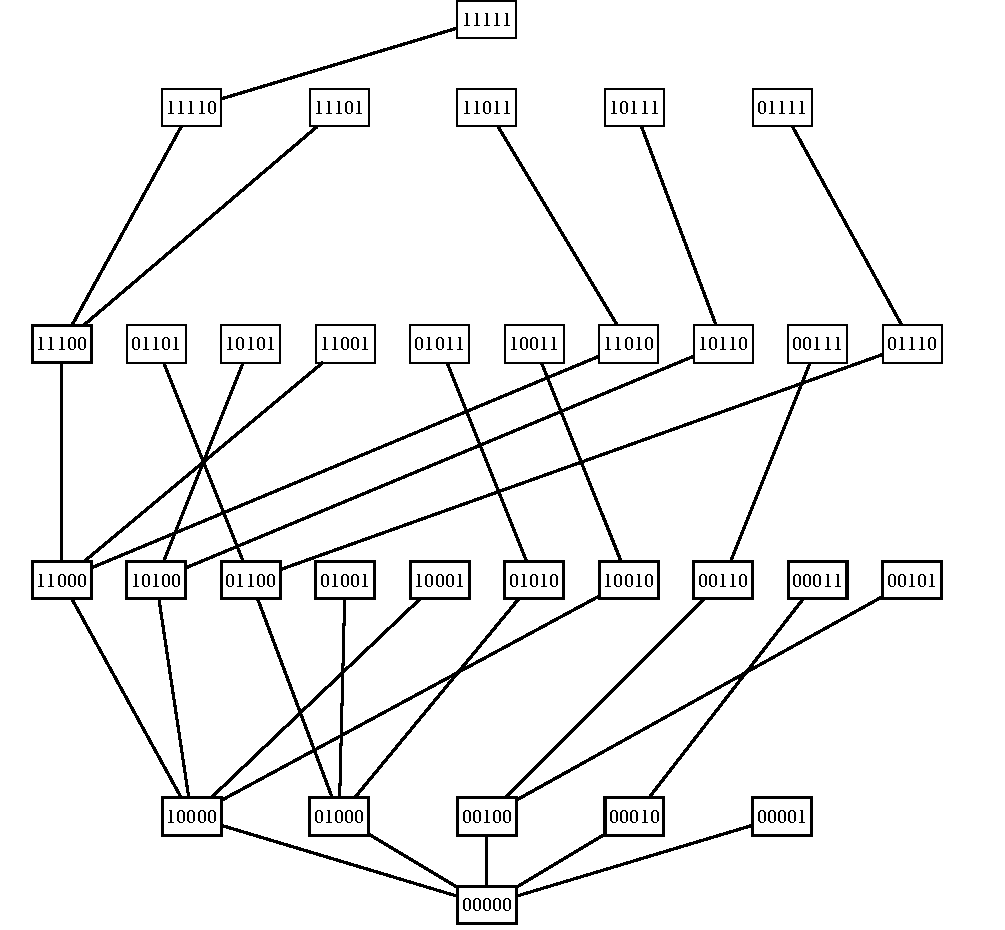
\includegraphics[clip=true]{pfs/ubb/ubb_tree.pdf}}
    \label{fig:ubb:tree} }
  \end{tabular}
\end{figure}  
\end{frame}

\begin{frame}{O algoritmo \algname{U-Curve-Branch-and-Bound}}
Este algoritmo busca o mínimo global ramificando na árvore como em uma
busca em profundidade e faz podas sempre que o custo aumenta.
\begin{figure}[!ht]
  \centering 
  \begin{tabular}{c c}
    \subfigure {\scalebox{0.3}{
     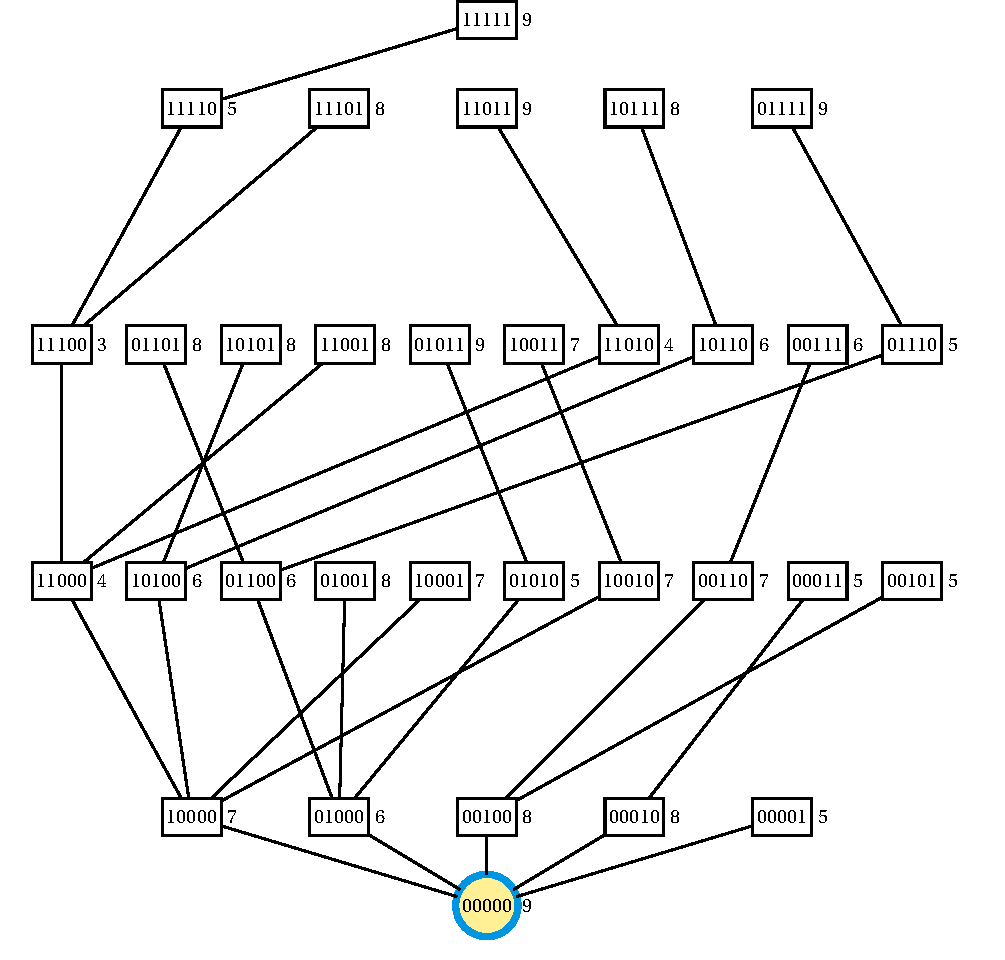
\includegraphics[clip=true]{pfs/ubb_run/b.pdf}}
     \label{fig:ubb:full} }
    & 
    \pause
    \subfigure {\scalebox{.3}{
    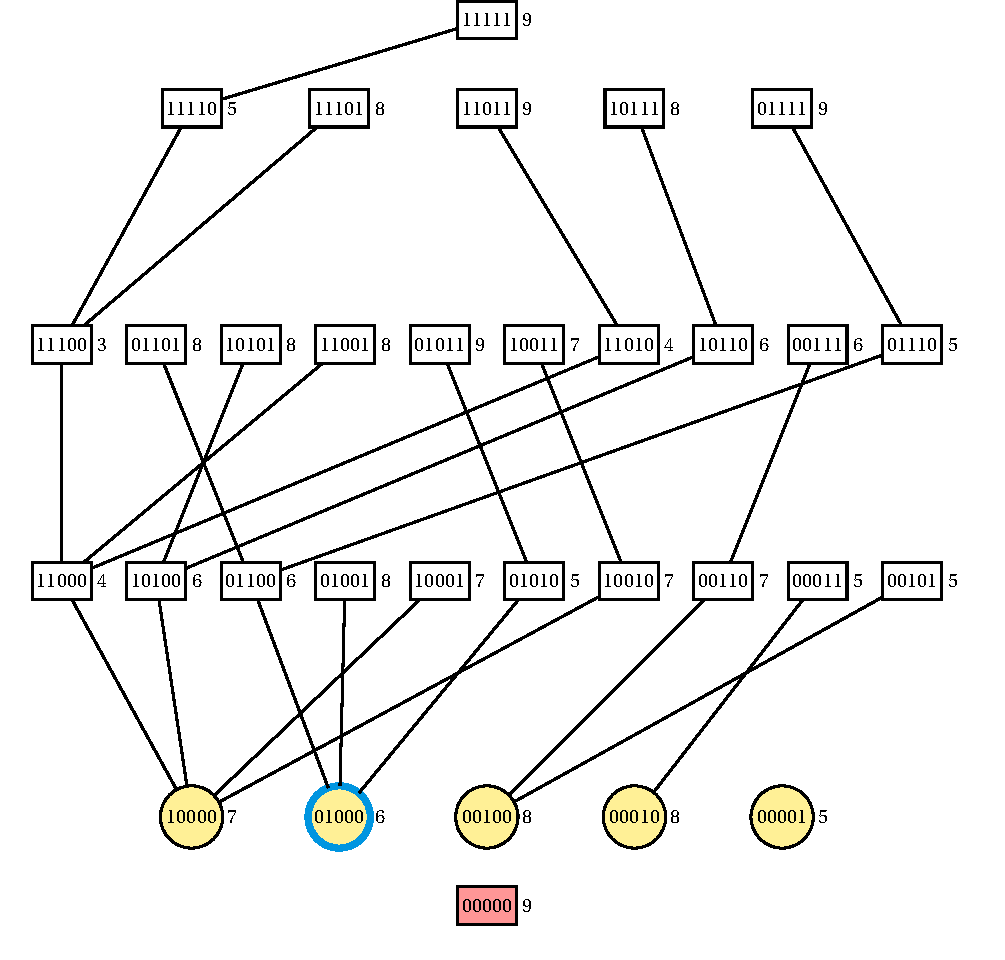
\includegraphics[clip=true]{pfs/ubb_run/c.pdf}}
    \label{fig:ubb:tree} }
  \end{tabular}
\end{figure}  
\end{frame}

\begin{frame}{O algoritmo \algname{U-Curve-Branch-and-Bound}}
\begin{figure}[!ht]
  \centering 
  \begin{tabular}{c c}
    \subfigure {\scalebox{0.3}{
     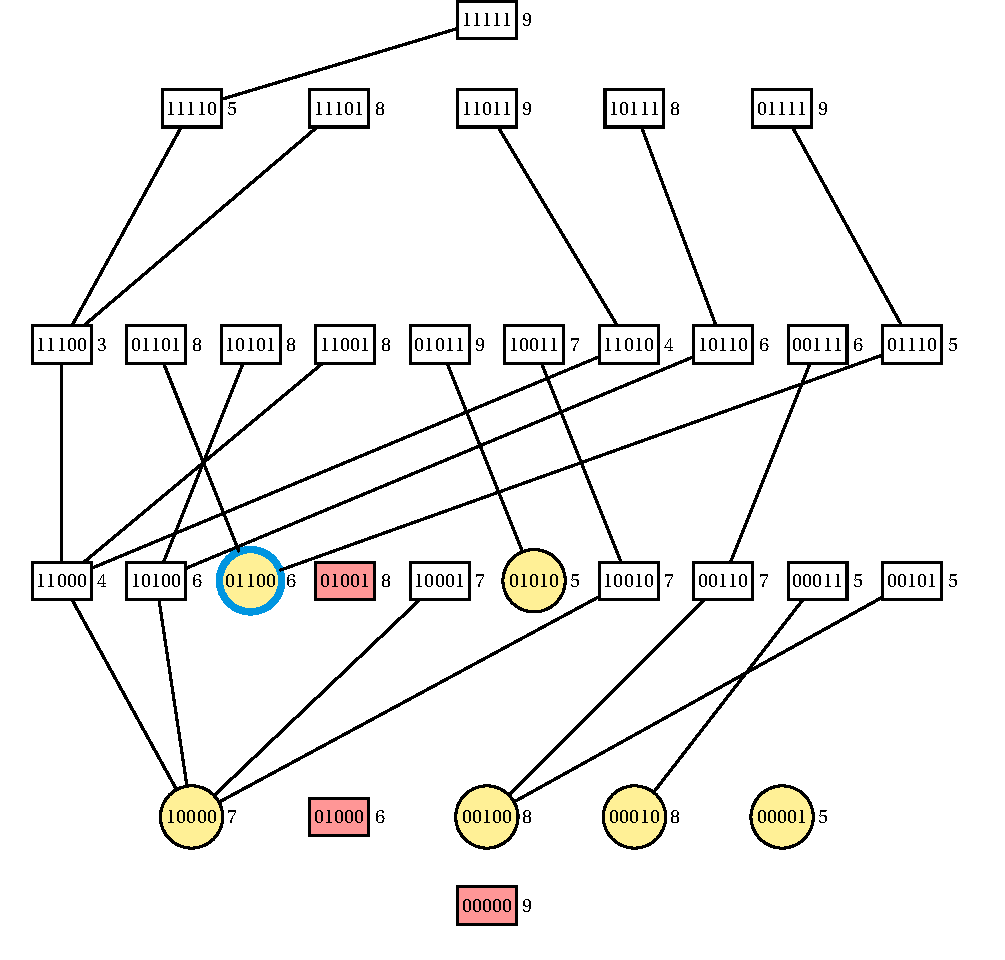
\includegraphics[clip=true]{pfs/ubb_run/d.pdf}}
     \label{fig:ubb:full} }
    \pause
    & 
    \subfigure {\scalebox{.3}{
    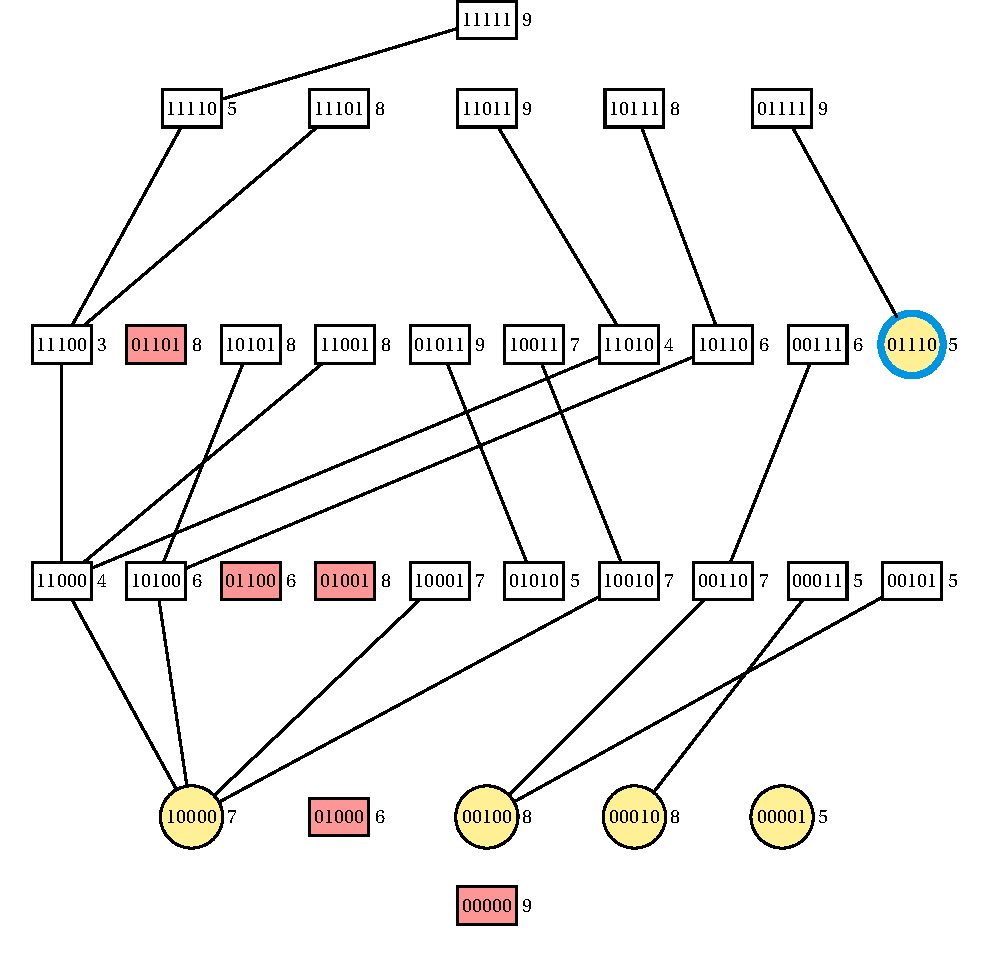
\includegraphics[clip=true]{pfs/ubb_run/e.pdf}}
    \label{fig:ubb:tree} }
  \end{tabular}
\end{figure}  
\pause
Note que se a condição de poda nunca é verdadeira, então o espaço
de busca inteiro é percorrido.
\end{frame}

\begin{frame}{O algoritmo \algname{Poset-Forest-Search}}
  Solução: percorrer o espaço de busca em duas direções.
  \pause
  %\vspace{1em}
  
  O algoritmo \algname{Poset-Fores-Search} (\algname{PFS}) pode fazer
  isso porque decompõe o espaço em duas árvores.
  \begin{figure}[!ht]
  \centering 
  \begin{tabular}{c c}
    \subfigure {\scalebox{0.28}{
     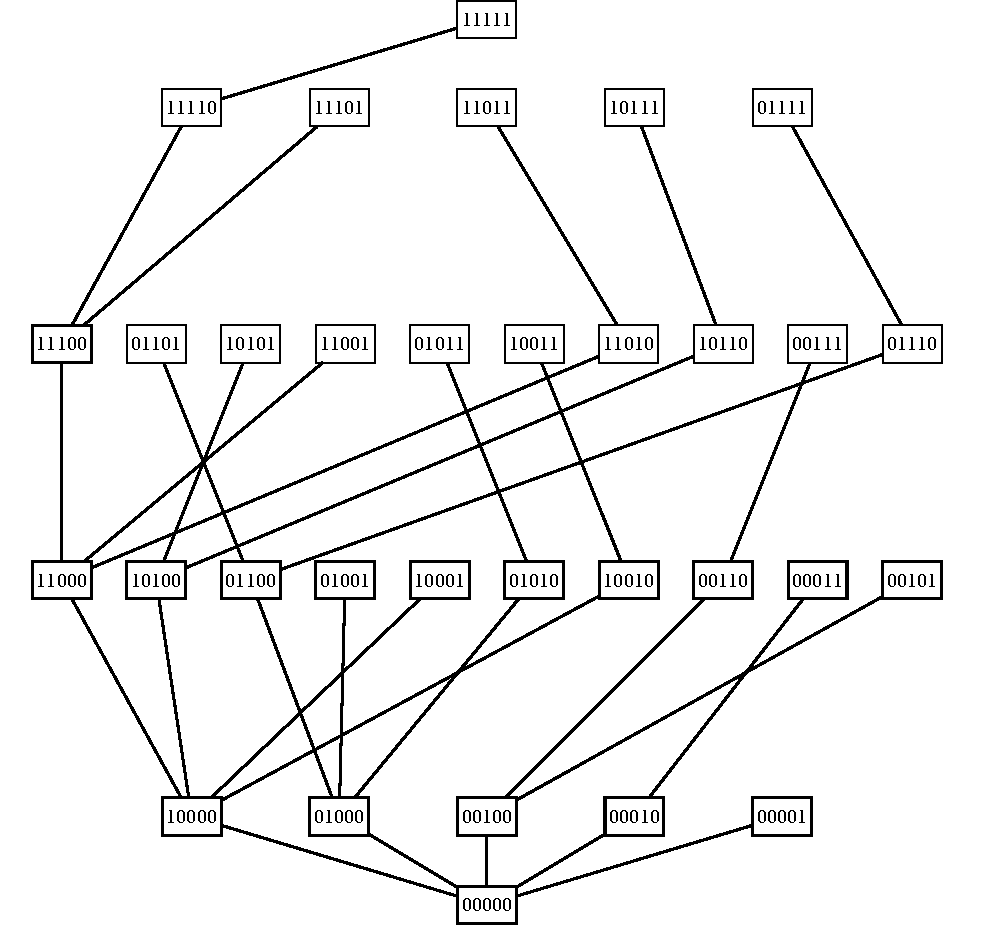
\includegraphics[clip=true]{pfs/pfs/lower_tree.pdf}}
     \label{fig:ubb:full} }
    \pause
    & 
    \subfigure {\scalebox{.28}{
    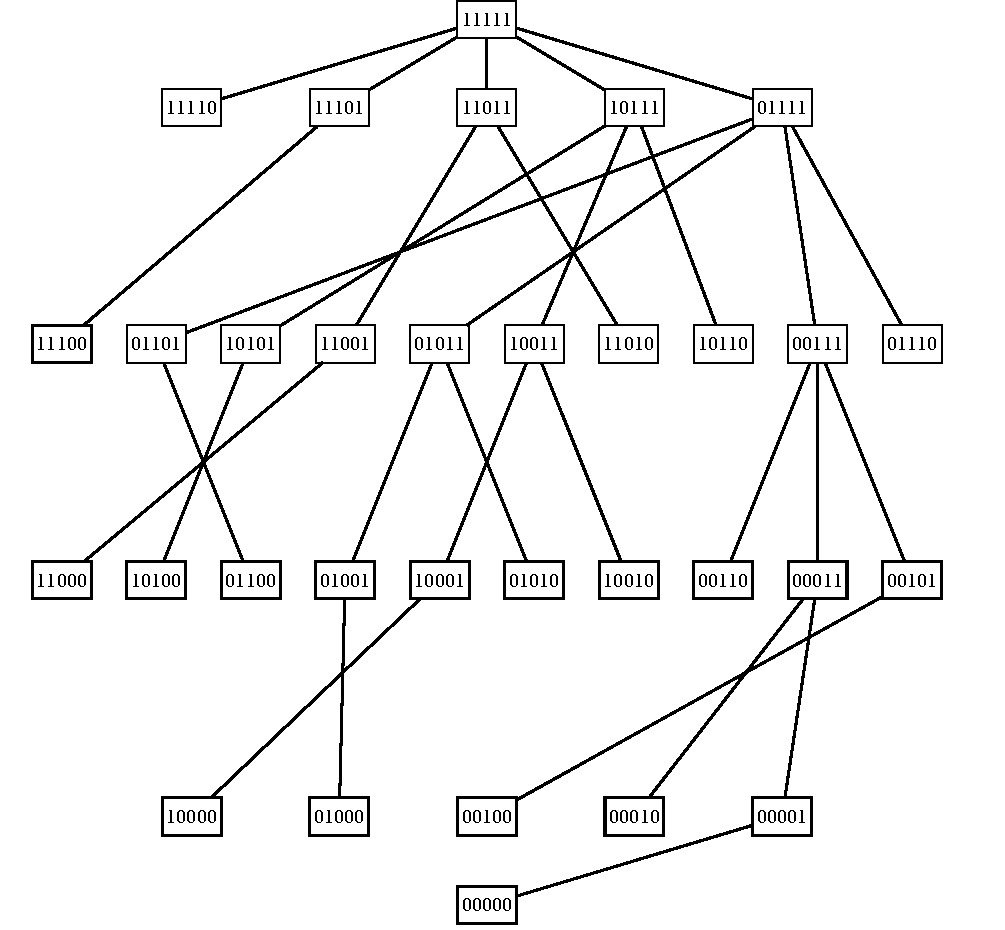
\includegraphics[clip=true]{pfs/pfs/upper_tree.pdf}}
    \label{fig:ubb:tree} }
  \end{tabular}
  \end{figure}  
\end{frame}

\begin{frame}{O algoritmo \algname{Poset-Forest-Search}}
  Problema: agora é necessário manter as duas árvores equivalentes,
  ou seja, representando o mesmo espaço de busca.
  \begin{figure}[!ht]
  \centering 
  \begin{tabular}{c c}
    \subfigure {\scalebox{0.28}{
     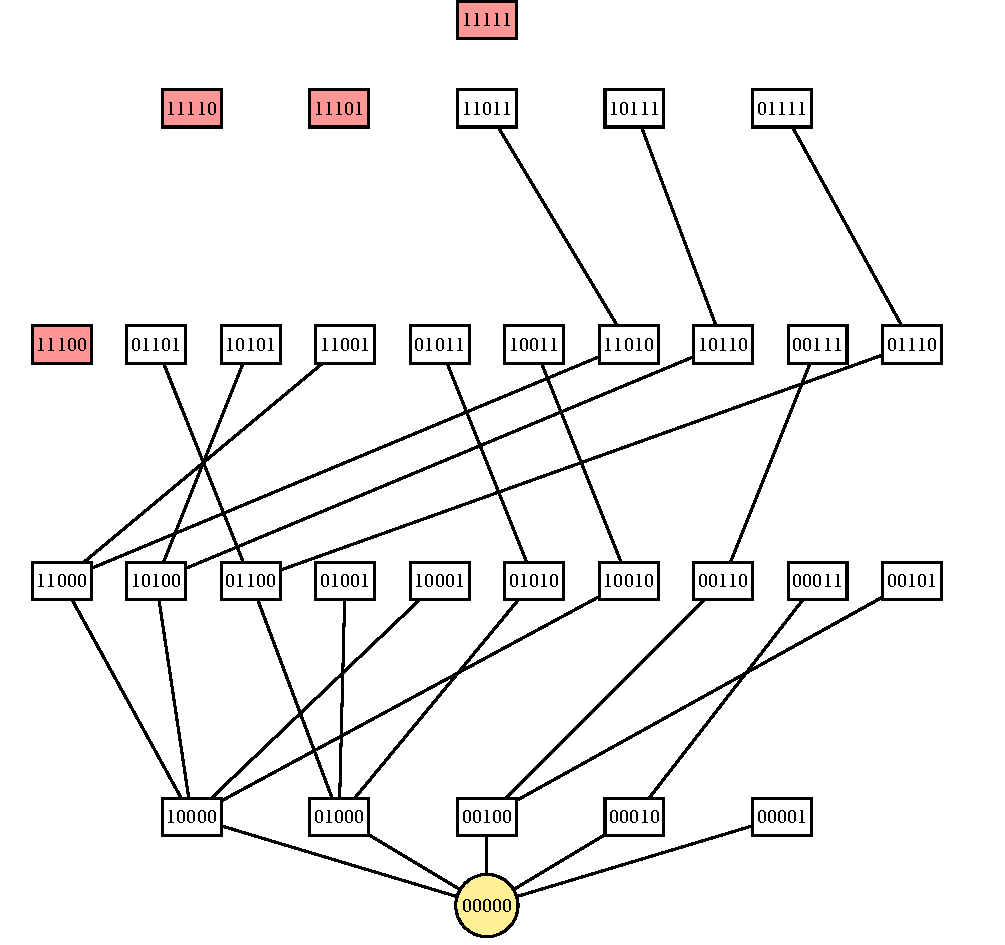
\includegraphics[clip=true]{pfs/pfs/forest/lower_tree.pdf}}
     \label{fig:ubb:full} }
    & 
    \pause
    \subfigure {\scalebox{.28}{
    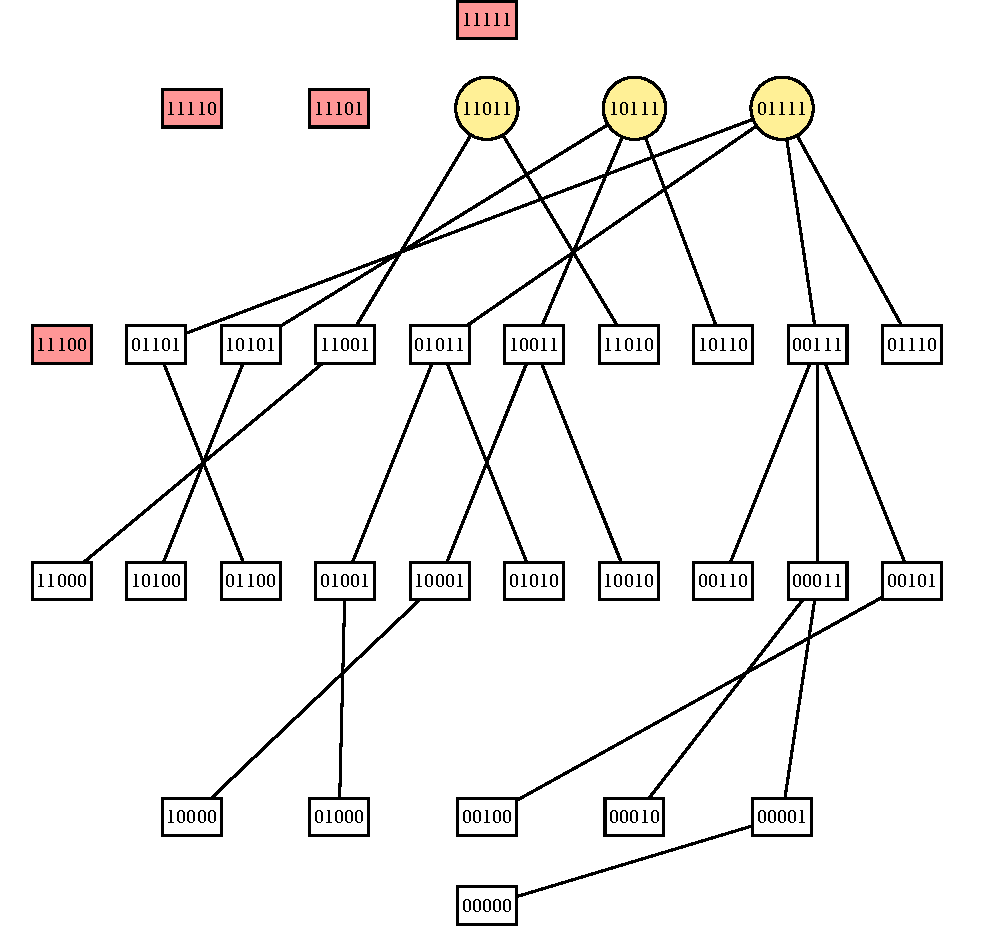
\includegraphics[clip=true]{pfs/pfs/forest/upper_tree.pdf}}
    \label{fig:ubb:tree} }
  \end{tabular}
  \end{figure}  
\end{frame}

\begin{frame}{O algoritmo \algname{Poset-Forest-Search}}
Podemos resumir o funcionamento do \algname{PFS} aos seguintes passos:
\pause
\begin{itemize}
  \item{Escolher uma direção de percorrimento}
  \pause
  \item{Percorrer uma cadeia da floresta escolhida}
  \pause
  \item{Sempre que a condição de poda for verdadeira:}
  \pause
    \begin{itemize}
    \item{Podar a floresta de percorrimento}
    \pause
    \item{Atualizar a floresta dual}
    \pause
    \end{itemize}
\end{itemize}
\end{frame}


%----------------------------------------------------------------------
\section{Melhoramentos ao \algname{Poset-Forest-Search}}


\begin{frame}{Melhoramentos na implementação atual do \algname{PFS}}
  O algoritmo implementado por Marcelo possui pontos que podiam ser
  explorados para se ter melhor desempenho computacional.
\end{frame}


\begin{frame}{Mudanças na escolha de raízes}
A implementação de Marcelo escolhia \alert{arbitrariamente} como raiz de
percorrimento a primeira quando ordenadas lexicograficamente.
\vspace{2em}\\
\pause
Propomos duas estratégias de escolhas:
\begin{itemize}
  \item{escolha aleatória e uniforme entre raízes;}
  \pause
  \item{escolha da raiz com maior sub-árvore.}
\end{itemize}
\end{frame}


\begin{frame}{Resultados da mudança de escolha de raízes}
Chamamos a variação do \algname{PFS} que escolhe raízes de maneira 
aleatória e identicamente provável de \algname{PFS-RAND}.
\pause
\begin{table}
\centering
\footnotesize
\label{tab:pfsrand_vs_pfs}
\resizebox{\columnwidth}{!}{%
\begin{tabular}{cc c cc c cc}
\toprule
\multicolumn{2}{c}{Instância} & \phantom{} & \multicolumn{2}{c}{Tempo de execução médio (s)}  & \phantom{} & \multicolumn{2}{c}{Número médio de cálculos de custo}\\
\cline{1-2}\cline{4-5}\cline{7-8}\\
$|S|$ & $2^{|S|}$ && \algname{PFS} & \algname{PFS\_RAND} && \algname{PFS} & \algname{PFS\_RAND} \\
% 10 &    1024 &&  0.013 $\pm$ 0.003 & 0.014 $\pm$ 0.003 &&   590.8 $\pm$ 198.5 & 599.5 $\pm$ 177.5 \\
% 11 &    2048 &&  0.019 $\pm$ 0.004 & 0.022 $\pm$ 0.007 &&   1114.8 $\pm$ 331.3 & 1090.1 $\pm$ 350.3 \\
% 12 &    4096 &&  0.029 $\pm$ 0.008 & 0.036 $\pm$ 0.013 &&   1848.6 $\pm$ 600.8 & 1835.7 $\pm$ 683.0 \\
% 13 &    8192 &&  0.060 $\pm$ 0.018 & 0.090 $\pm$ 0.039 &&   4314.4 $\pm$ 1496.4 & 4201.1 $\pm$ 1580.7 \\
% 14 &   16384 &&  0.100 $\pm$ 0.041 & 0.191 $\pm$ 0.110 &&   7323.4 $\pm$ 3318.9 & 7333.8 $\pm$ 3161.0 \\
    15 &   32768 &&  \textbf{0.180 $\pm$ 0.076} & 0.453 $\pm$ 0.311 &&   12958.1 $\pm$ 5654.0 & \textbf{12807.5 $\pm$ 5753.7} \\
16 &   65536 &&  \textbf{0.406 $\pm$ 0.185} & 1.715 $\pm$ 1.400 &&   27573.8 $\pm$ 12459.5 & \textbf{27036.9 $\pm$ 12687.5} \\
17 &  131072 &&  \textbf{0.717 $\pm$ 0.397} & 5.416 $\pm$ 5.266 &&   48176.2 $\pm$ 26938.3 & \textbf{47852.1 $\pm$ 26427.6} \\
18 &  262144 &&  \textbf{1.325 $\pm$ 0.754} & 15.890 $\pm$ 17.726 &&   84417.9 $\pm$ 48587.7 & \textbf{84025.0 $\pm$ 48882.4} \\
19 &  524288 &&  \textbf{2.771 $\pm$ 1.603} & 69.600 $\pm$ 82.342 &&   167659.1 $\pm$ 99686.7 & \textbf{164612.1 $\pm$ 102018.3} \\
\bottomrule
\end{tabular}%
}
\end{table}
\end{frame}


\begin{frame}{Resultados da mudança de escolha de raízes}
Chamamos a variação do \algname{PFS} que escolhe as raízes com maior
sub-árvore de \algname{PFS-LEFTMOST}.
\pause
\begin{table}
\centering
\resizebox{\columnwidth}{!}{%
\begin{tabular}{cc c cc c cc}
\toprule
\multicolumn{2}{c}{Instância} & \phantom{} & \multicolumn{2}{c}{Tempo de execução médio (s)}  & \phantom{} & \multicolumn{2}{c}{Número médio de cálculos de custo}\\
\cline{1-2}\cline{4-5}\cline{7-8}\\
$|S|$ & $2^{|S|}$ && \algname{PFS} & \algname{PFS\_LEFTMOST} && \algname{PFS} & \algname{PFS\_LEFTMOST} \\
% 10 &    1024 \textbf{&&  0.013 $\pm$ 0}.002 & 0.023 $\pm$ 0.004 &&  606.1 $\pm$ 133.5 & 665.0 $\pm$ 165.8 \\
% 11 &    2048 \textbf{&&  0.020 $\pm$ 0}.004 & 0.042 $\pm$ 0.010 &&  1122.1 $\pm$ 351.2 & 1316.6 $\pm$ 382.2 \\
% 12 &    4096 \textbf{&&  0.032 $\pm$ 0}.008 & 0.078 $\pm$ 0.024 &&  2183.7 $\pm$ 733.2 & 2515.8 $\pm$ 871.3 \\
% 13 &    8192 \textbf{&&  0.054 $\pm$ 0}.017 & 0.160 $\pm$ 0.061 &&  3887.7 $\pm$ 1389.9 & 4716.8 $\pm$ 1777.8 \\
% 14 &   16384 \textbf{&&  0.107 $\pm$ 0}.034 & 0.345 $\pm$ 0.133 &&  7851.2 $\pm$ 2793.0 & 9506.8 $\pm$ 3673.9 \\
15 &   32768 &&  \textbf{0.196 $\pm$ 0.085} & 0.672 $\pm$ 0.274 &&  \textbf{13780.3 $\pm$ 6049.9} & 17071.6 $\pm$ 7005.1 \\
16 &   65536 &&  \textbf{0.348 $\pm$ 0.189} & 1.271 $\pm$ 0.661 &&  \textbf{24106.5 $\pm$ 13159.9} & 30055.6 $\pm$ 15363.6 \\
17 &  131072 &&  \textbf{0.785 $\pm$ 0.361} & 3.137 $\pm$ 1.476 &&  \textbf{52369.0 $\pm$ 24751.2} & 67585.6 $\pm$ 30978.4 \\
18 &  262144 &&  \textbf{1.445 $\pm$ 0.657} & 6.146 $\pm$ 3.032 &&  \textbf{92095.9 $\pm$ 42566.6} & 120635.7 $\pm$ 58039.0 \\
19 &  524288 &&  \textbf{3.298 $\pm$ 1.883} & 13.881 $\pm$ 7.595 &&  \textbf{199151.0 $\pm$ 112167.8} & 256078.6 $\pm$ 135958.4 \\
\bottomrule 
\end{tabular}%
}
\end{table}
\end{frame}


\begin{frame}{Melhoramentos na estrutura de armazenamento de raízes}
  Mudamos a implementação de Marcelo para usar diagramas de decisão
  binários ordenados (OBDDs).
  \pause
  \begin{figure}[]
  \centering 
  \begin{tabular}{c c}
    \subfigure {\scalebox{.5}{
     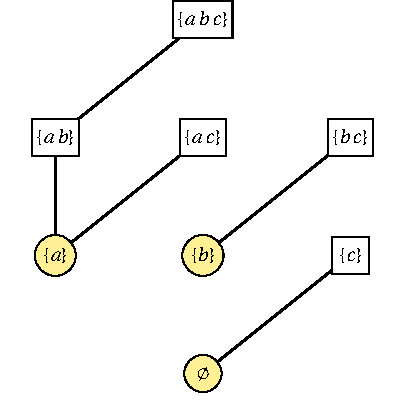
\includegraphics[clip=true]{pfs/obdd/lattice.pdf}}
     \label{fig:pfs:obdd:A} }
      & 
      \subfigure {\scalebox{.65}{
    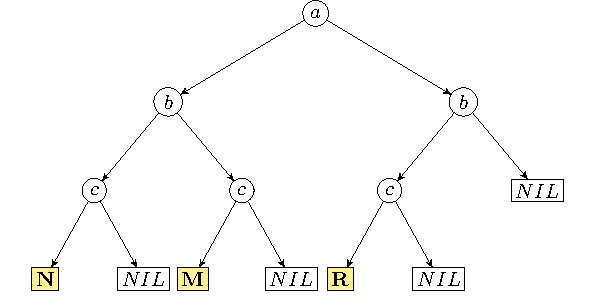
\includegraphics[clip=true]{pfs/obdd/obdd.pdf}}
    \label{fig:pfs:obdd:B} }
  \end{tabular}
  \end{figure}
\end{frame}


\begin{frame}{Resultados da mudança de estrutura para armazenamento de raízes}
Chamamos de \algname{OPFS} o algoritmo que usa OBDDs para armazenamento
de raízes.
\begin{table}
\centering
\resizebox{\columnwidth}{!}{
\begin{tabular}{cc c cc c cc}
\toprule
\multicolumn{2}{c}{Instância} & \phantom{} & \multicolumn{2}{c}{Tempo de execução médio (s)}  & \phantom{} & \multicolumn{2}{c}{Número médio de cálculos de custo}\\
\cline{1-2}\cline{4-5}\cline{7-8}\\
$|S|$ & $2^{|S|}$ && \algname{PFS} & \algname{OPFS} && \algname{PFS} & \algname{OPFS} \\
% 10 &    1024 &&  0.013 $\pm$ 0.003 & 0.018 $\pm$ 0.003 &&  598.0 $\pm$ 192.8 & 635.5 $\pm$ 171.9 \\
% 11 &    2048 \textbf{&&  0.020 $\pm$ 0}.004 & 0.029 $\pm$ 0.007 &&  1152.1 $\pm$ 314.7 \textbf{& 1117.9 $\pm$ 336}.4 \\
% 12 &    4096 \textbf{&&  0.031 $\pm$ 0}.010 & 0.049 $\pm$ 0.013 &&  2024.1 $\pm$ 751.6 \textbf{& 2048.2 $\pm$ 700}.9 \\
% 13 &    8192 \textbf{&&  0.057 $\pm$ 0}.017 & 0.097 $\pm$ 0.033 &&  3996.3 $\pm$ 1431.6 \textbf{& 3973.4 $\pm$ 1462}.6 \\
% 14 &   16384 \textbf{&&  0.094 $\pm$ 0}.038 & 0.171 $\pm$ 0.063 &&  6634.8 $\pm$ 2944.0 \textbf{& 6906.5 $\pm$ 2786}.5 \\
% 15 &   32768 \textbf{&&  0.182 $\pm$ 0}.079 & 0.323 $\pm$ 0.156 &&  13140.1 $\pm$ 6020.6 \textbf{& 12711.2 $\pm$ 6319}.7 \\
% 16 &   65536 \textbf{&&  0.370 $\pm$ 0}.169 & 0.660 $\pm$ 0.314 &&  25658.2 $\pm$ 11606.7 \textbf{& 25303.4 $\pm$ 12169}.5 \\
% 17 &  131072 \textbf{&&  0.819 $\pm$ 0}.370 & 1.480 $\pm$ 0.665 &&  53344.9 $\pm$ 24350.4 \textbf{& 53217.2 $\pm$ 24154}.5 \\
% 18 &  262144 \textbf{&&  1.515 $\pm$ 0}.905 & 2.736 $\pm$ 1.626 &&  94677.6 $\pm$ 54496.3 \textbf{& 94079.4 $\pm$ 55435}.6 \\
19 &  524288 &&  \textbf{2.612 $\pm$ 1.869} & 4.818 $\pm$ 3.355 &&  156150.5 $\pm$ 107369.8 & \textbf{156021.8 $\pm$ 107516.8} \\
20 & 1048576 &&  \textbf{6.085 $\pm$ 3.900} & 11.550 $\pm$ 7.661 &&  344144.1 $\pm$ 212627.1 & \textbf{343229.2 $\pm$ 212624.4} \\
21 & 2097152 &&  \textbf{11.416 $\pm$ 8.296} & 21.818 $\pm$ 16.269 &&  616936.2 $\pm$ 436491.2 & \textbf{613526.2 $\pm$ 438580.0} \\
22 & 4194304 &&  \textbf{19.950 $\pm$ 17.799} & 42.112 $\pm$ 45.109 &&  960842.2 $\pm$ 785137.2 & \textbf{959905.4 $\pm$ 783257.3} \\
23 & 8388608 &&  \textbf{42.792 $\pm$ 35.622} & 87.262 $\pm$ 90.579 &&  \textbf{2053472.4 $\pm$ 1690882.1} & 2060184.5 $\pm$ 1682011.0 \\
% 24 & 16777216 &&  85.646 $\pm$ 79.186 & 149.567 $\pm$ 108.104 &&  4080290.8 $\pm$ 3166258.4 & 4100480.6 $\pm$ 3141423.9 \\
\bottomrule 
\end{tabular}%
}
\end{table}
\end{frame}


\begin{frame}{Paralelização do \algname{PFS}}
Implementamos também uma versão paralela do algoritmo \algname{PFS}.
\vspace{1em}
\pause\\

Entretanto, a etapa de atualização da floresta dual é complicada e pode 
gerar condições de corrida, o que deixou a paralelização complicada.
\end{frame}

\begin{frame}{O algoritmo \algname{UBB-PFS}}
Este algoritmo é uma nova alternativa paralela que é dividida em duas
partes:
\vspace{1em}
\pause\\
\begin{itemize}
  \item{Percorrimento sequencial: idêntico ao \algname{UBB} deve criar
    sub-árvores no espaço enquanto faz uma ramificação do tipo
    busca em profundidade.}
  \pause
  \item{Solução em paralelo: cada sub-árvore gerada na etapa de 
    ramificação deve ser resolvida por uma chamada do \algname{PFS}.}
\end{itemize}
\end{frame}


\begin{frame}{Resultados do \algname{UBB-PFS}}
O \algname{UBB-PFS} foi mais rápido do que o \algname{PFS}.
\begin{table}
\centering
\footnotesize
\resizebox{\columnwidth}{!}{%
\begin{tabular}{cc c ccc}
\toprule
\multicolumn{2}{c}{Instância} & \phantom{} & \multicolumn{3}{c}{Tempo de execução médio (s)}\\
\cline{1-2}\cline{4-6}\\
$|S|$ & $2^{|S|}$ && \algname{UBB} & \algname{PFS} & \algname{UBB-PFS}  \\
%10 &    1024 &&  0.006 $\pm$ 0.001 & 0.011 $\pm$ 0.002 & 0.023 $\pm$ 0.004 \\
%11 &    2048 &&  0.007 $\pm$ 0.001 & 0.017 $\pm$ 0.004 & 0.026 $\pm$ 0.004 \\
%12 &    4096 &&  0.010 $\pm$ 0.003 & 0.029 $\pm$ 0.009 & 0.034 $\pm$ 0.006 \\
%13 &    8192 &&  0.013 $\pm$ 0.006 & 0.047 $\pm$ 0.016 & 0.044 $\pm$ 0.011 \\
%14 &   16384 &&  0.024 $\pm$ 0.013 & 0.094 $\pm$ 0.034 & 0.068 $\pm$ 0.023 \\
%15 &   32768 &&  0.043 $\pm$ 0.026 & 0.186 $\pm$ 0.074 & 0.113 $\pm$ 0.042 \\
%16 &   65536 &&  0.083 $\pm$ 0.060 & 0.339 $\pm$ 0.168 & 0.187 $\pm$ 0.082 \\
% 17 &  131072 &&  0.161 $\pm$ 0.122 & 0.650 $\pm$ 0.347 & 0.326 $\pm$ 0.175 \\
% 18 &  262144 &&  0.321 $\pm$ 0.233 & 1.482 $\pm$ 0.768 & 0.703 $\pm$ 0.380 \\
% 19 &  524288 &&  0.620 $\pm$ 0.447 & 2.711 $\pm$ 1.562 & 1.309 $\pm$ 0.729 \\
20 & 1048576 &&  \textbf{1.312 $\pm$ 0.970} & 5.007 $\pm$ 3.302 & 2.478 $\pm$ 1.547 \\
21 & 2097152 &&  \textbf{2.494 $\pm$ 1.893} & 11.125 $\pm$ 6.749 & 5.458 $\pm$ 3.294 \\
22 & 4194304 &&  \textbf{4.589 $\pm$ 4.122} & 19.085 $\pm$ 15.147 & 8.832 $\pm$ 6.846 \\
23 & 8388608 &&  \textbf{12.228 $\pm$ 7.922} & 40.323 $\pm$ 29.649 & 18.891 $\pm$ 12.786 \\
24 & 16777216 &&  \textbf{24.273 $\pm$ 16.277} & 113.332 $\pm$ 76.688 & 67.178 $\pm$ 46.516 \\
\bottomrule
\end{tabular} 
}
\end{table}
\end{frame}


\begin{frame}{Resultados do \algname{UBB-PFS}}
E computou menos a função custo do que o \algname{UBB}.
\begin{table}
\centering
\footnotesize
\resizebox{\columnwidth}{!}{%
\begin{tabular}{cc c ccc}
\toprule
\multicolumn{2}{c}{Instância} & \phantom{} & \multicolumn{3}{c}{Número médio de cálculos de custo}\\
\cline{1-2}\cline{4-6} \\
$|S|$ & $2^{|S|}$ && UBB & PFS & UBB-PFS  \\
%10 &    1024  && 699.4 $\pm$ 361.3 & 611.3 $\pm$ 178.8 & 634.7 $\pm$ 209.8 \\
%11 &    2048  && 1217.2 $\pm$ 747.1 & 1145.4 $\pm$ 358.9 & 1178.8 $\pm$ 484.1 \\
%12 &    4096  && 2898.0 $\pm$ 1380.4 & 2103.1 $\pm$ 793.6 & 2363.0 $\pm$ 760.4 \\
%13 &    8192  && 4422.6 $\pm$ 3293.8 & 3650.9 $\pm$ 1371.9 & 3934.4 $\pm$ 1487.7 \\
%14 &   16384  && 10089.4 $\pm$ 6452.1 & 7536.3 $\pm$ 2926.1 & 8012.2 $\pm$ 3387.4 \\
%15 &   32768  && 19097.5 $\pm$ 12793.8 & 14546.5 $\pm$ 6081.0 & 15299.2 $\pm$ 6598.4 \\
%16 &   65536  && 37663.1 $\pm$ 28321.2 & 25744.0 $\pm$ 12795.4 & 27028.4 $\pm$ 13031.9 \\
% 17 &  131072  && 73373.3 $\pm$ 55994.3 & 46808.9 $\pm$ 24533.5 & 49348.6 $\pm$ 24556.7 \\
% 18 &  262144  && 150035.2 $\pm$ 108299.3 & 103166.6 $\pm$ 52464.7 & 105306.4 $\pm$ 53472.0 \\
% 19 &  524288  && 292561.2 $\pm$ 210771.2 & 183125.7 $\pm$ 104965.4 & 189545.7 $\pm$ 102145.9 \\
% 20 & 1048576  && 617049.5 $\pm$ 450468.2 & 323097.4 $\pm$ 213634.3 & 340694.2 $\pm$ 202389.6 \\
21 & 2097152  && 1172641.6 $\pm$ 879148.5 & \textbf{691991.3 $\pm$ 413262.9} & 704790.2 $\pm$ 407143.8 \\
22 & 4194304  && 2099973.2 $\pm$ 1863285.8 & \textbf{1133395.1 $\pm$ 874492.0} & 1156564.2 $\pm$ 862152.0 \\
23 & 8388608  && 5435778.8 $\pm$ 3468245.3 & \textbf{2276694.5 $\pm$ 1621342.2} & 2345648.2 $\pm$ 1558258.5 \\
24 & 16777216 && 10146842.9 $\pm$ 6673018.3 & \textbf{5527504.2 $\pm$ 3413432.3} & 5609052.7 $\pm$ 3337059.1 \\
\bottomrule
\end{tabular}
}
\end{table}
\end{frame}


% ----------------------------------------------------------------------
\section{O algoritmo \algname{Parallel-U-Curve-Search}}

\begin{frame}{Ideia do \algname{Parallel-U-Curve-Search} (\algname{PUCS})}
    Um algoritmo de fácil paralelização e pouco entrelace de linhas
    de processamento, \pause e que também distribua o trabalho em partes
    de tamanho parecido.\pause \\
    \vspace{1em}
    Fazemos isso ao definir um particionamento do espaço.
\begin{figure}[!ht]
  \centering 
  \begin{tabular}{c c}
    \subfigure {\scalebox{0.23}{
    \includegraphics[clip=true]{pucs/partition/full_lattice.pdf}}}
    &
    \subfigure {\scalebox{0.23}{
    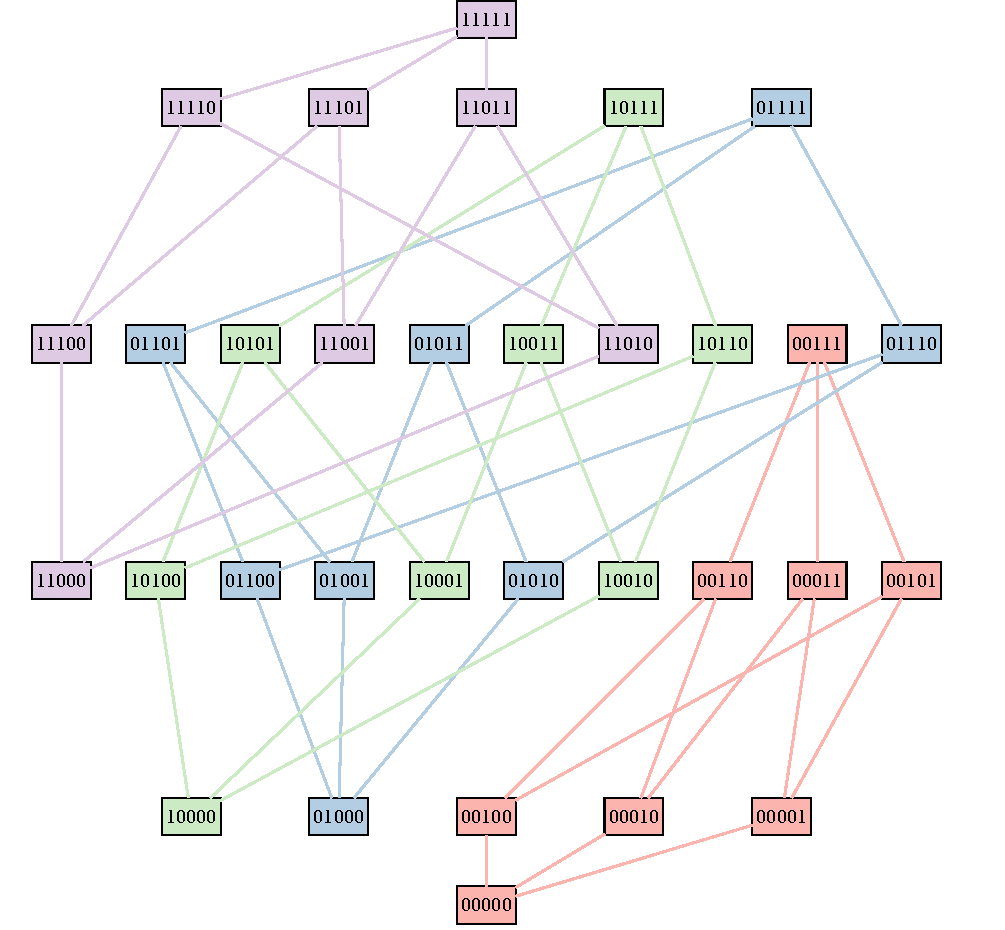
\includegraphics[clip=true]{pucs/partition/all_parts.pdf}}}\\
  \end{tabular}
\end{figure}
\end{frame}


\begin{frame}{Particionamento do espaço de busca}
Para particionar o espaço, escolhemos um conjunto arbitrário de 
variáveis $S'$. \pause

Agora, definimos a relação de equivalência para os conjuntos de 
características: \\
\begin{center}
$
\begin{aligned}
    X \sim Y \iff (X \cap S') = (Y \cap S')
\end{aligned}
$
\end{center}
\end{frame}

\begin{frame}{Estrutura recursiva do problema}
    Se representamos cada parte por um subconjunto de características de
    $S'$, então temos um reticulado Booleano de partes. Chamamos este
    reticulado de \alert{reticulado externo}.
    \vspace{1em}\\
    \pause
    Se representamos, cada nó de uma parte por um subconjunto de 
    características de $S - S'$, então temos um reticulado Booleano
    de nós de uma parte. Chamamos este reticulado de \alert{reticulado
    interno}.
\end{frame}

\begin{frame}{Estrutura recursiva do problema}
    \begin{figure}
    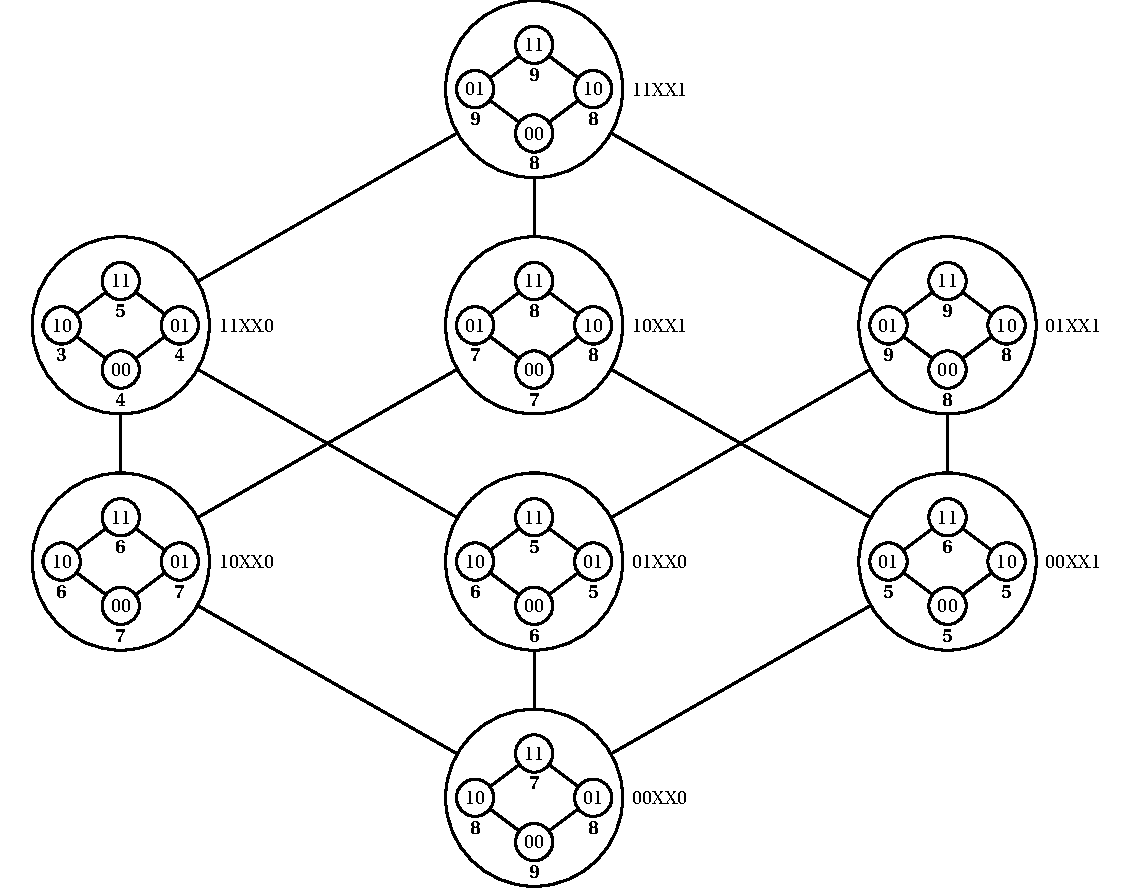
\includegraphics[clip=true, width=0.68\textwidth]{pucs/sample_run/A.pdf}
    \end{figure}
\end{frame}

\begin{frame}{Dinâmica}
    Podemos resumir a dinâmica deste algoritmo nos passos:
    \begin{itemize}
    \item{passeio aleatório no reticulado externo, com podas;}
    \item{solução de partes não podadas;}
    \item{união de respostas das partes.}
    \end{itemize}
\end{frame}

\begin{frame}{Pontas de um reticulado}
    Se $X$ é um conjunto maximal em um reticulado Booleano, isto é,
    $Y \supseteq X \iff X = Y$, então $X$ é \alert{ponta de cima} do
    reticulado.
    \vspace{1em}\pause \\

    Se $X$ é conjunto minimal, isto é, $Y \subseteq X \iff X = Y$, então
    $X$ é \alert{ponta de baixo} do reticulado.
\end{frame}

\begin{frame}{Condições de poda}
    Sejam $P$ e $Q$ duas partes adjacentes, sendo que $Q \subseteq P$.
    \pause
    \begin{mydefinition}[Condição de poda inferior do \algname{PUCS}]
        Se o custo da ponta de cima de $Q$ é maior do que a ponta de 
        cima de $P$, então nenhuma das partes abaixo de $Q$ contém o 
        mínimo global.
    \end{mydefinition}
    \pause
    \begin{mydefinition}[Condição de poda superior do \algname{PUCS}]
        Se o custo da ponta de baixo de $P$ é maior do que a ponta de 
        baixo de $P$, então nenhuma das partes acima de $Q$ contém o 
        mínimo global.
    \end{mydefinition}
\end{frame}

\begin{frame}{Simulação de execução}
    \begin{figure}[!ht]
    \begin{center}
    \begin{tabular}{l r}
    \centering
    \subfigure{
        \label{fig:pucs:example:lattice}
        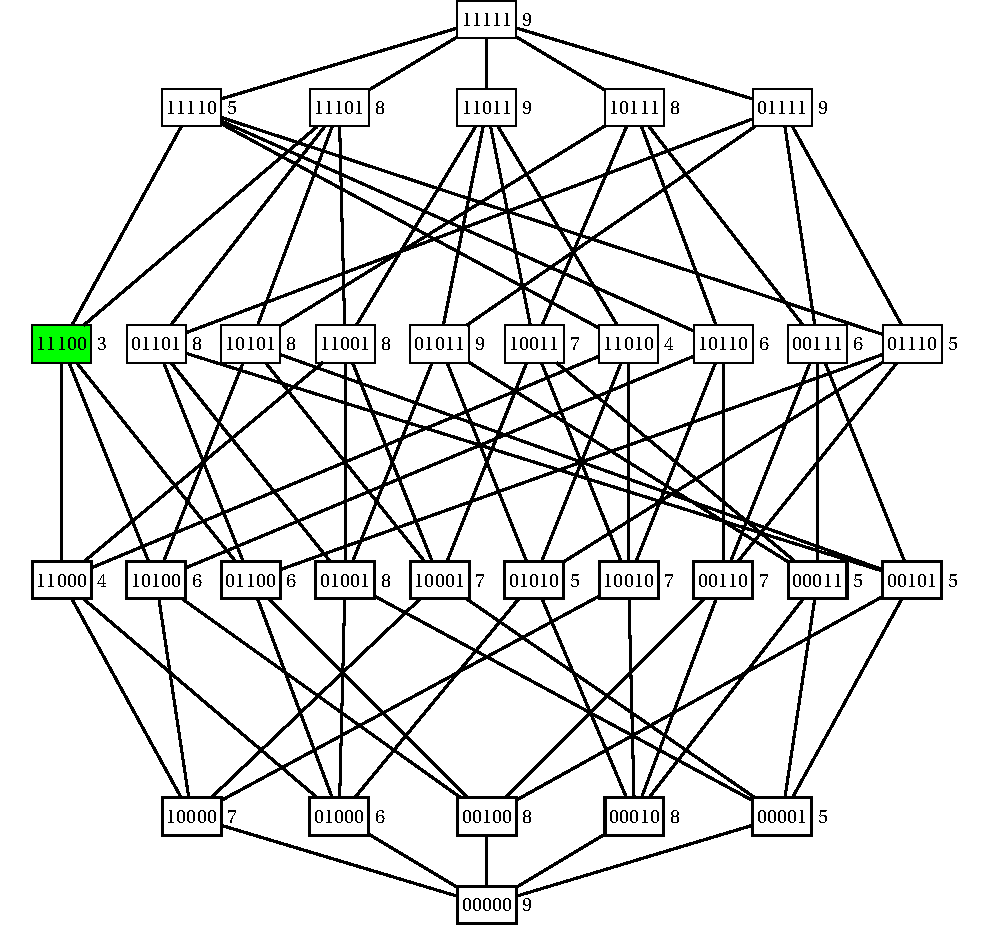
\includegraphics[clip=true, width=0.48\textwidth]{pucs/sample_run/Boolean_lattice.pdf}
    }
    &
    \subfigure{
        \label{fig:pucs:example:A}
        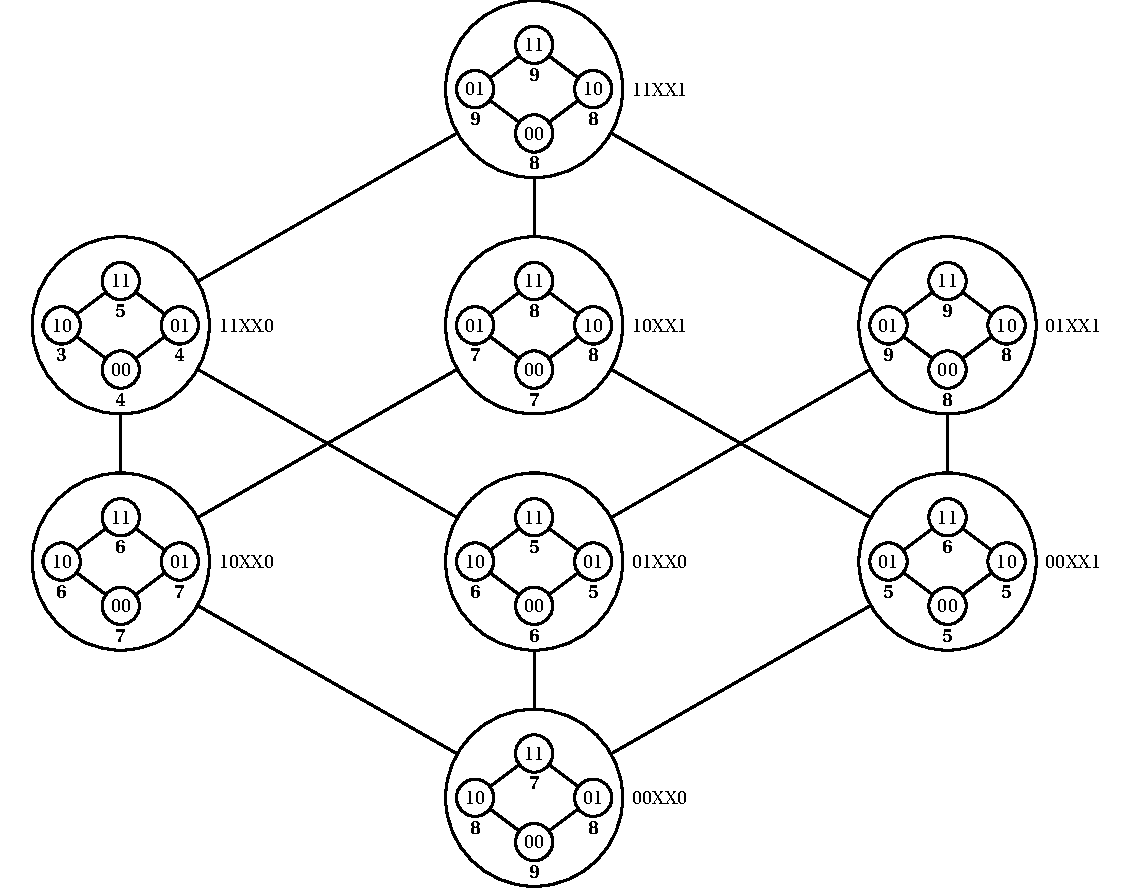
\includegraphics[clip=true, width=0.48\textwidth]{pucs/sample_run/A.pdf}
    }
    \end{tabular}   
    \end{center}
\end{figure}
\end{frame}

\begin{frame}{Simulação de execução}
    \begin{figure}[!ht]
    \begin{center}
    \begin{tabular}{l r}
    \centering
    \subfigure {
        \label{fig:pucs:example:B}
        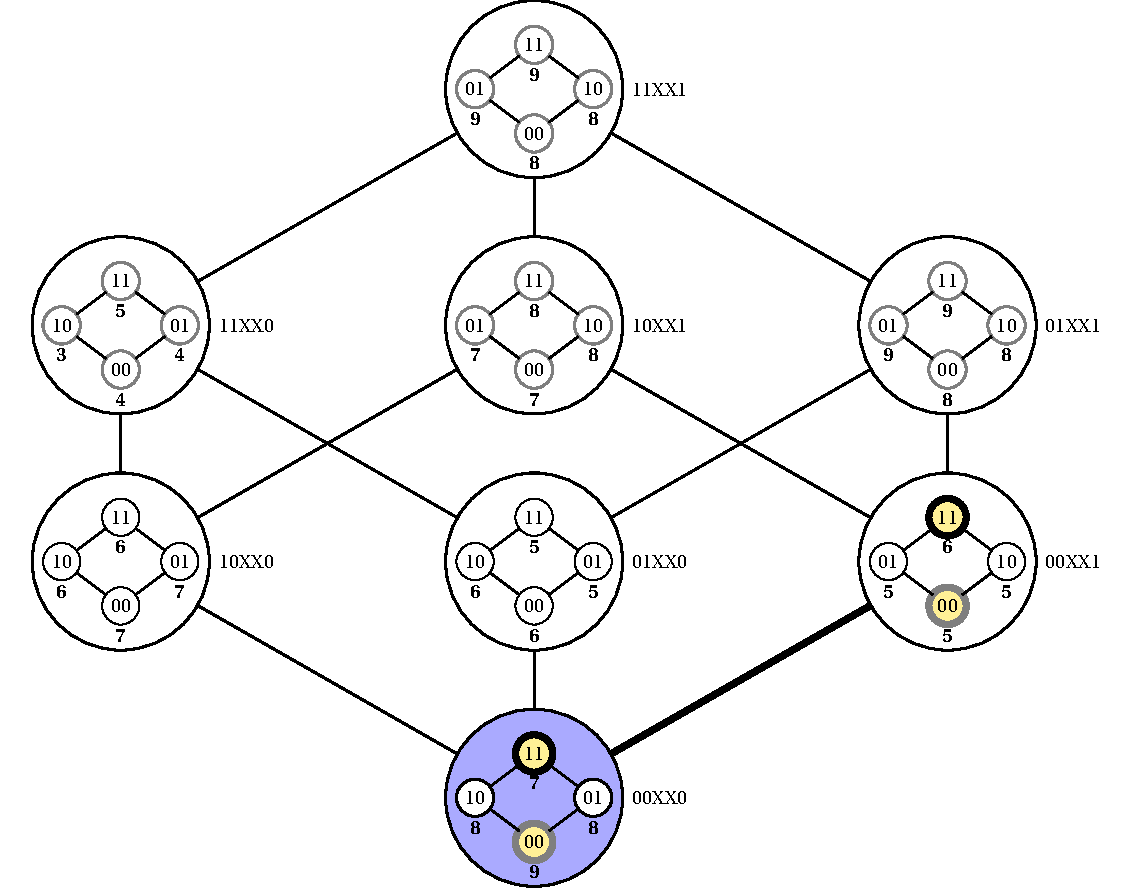
\includegraphics[ clip=true, width=0.4\textwidth]{pucs/sample_run/B.pdf}
    } \pause
    &
    \subfigure {
        \label{fig:pucs:example:C}
        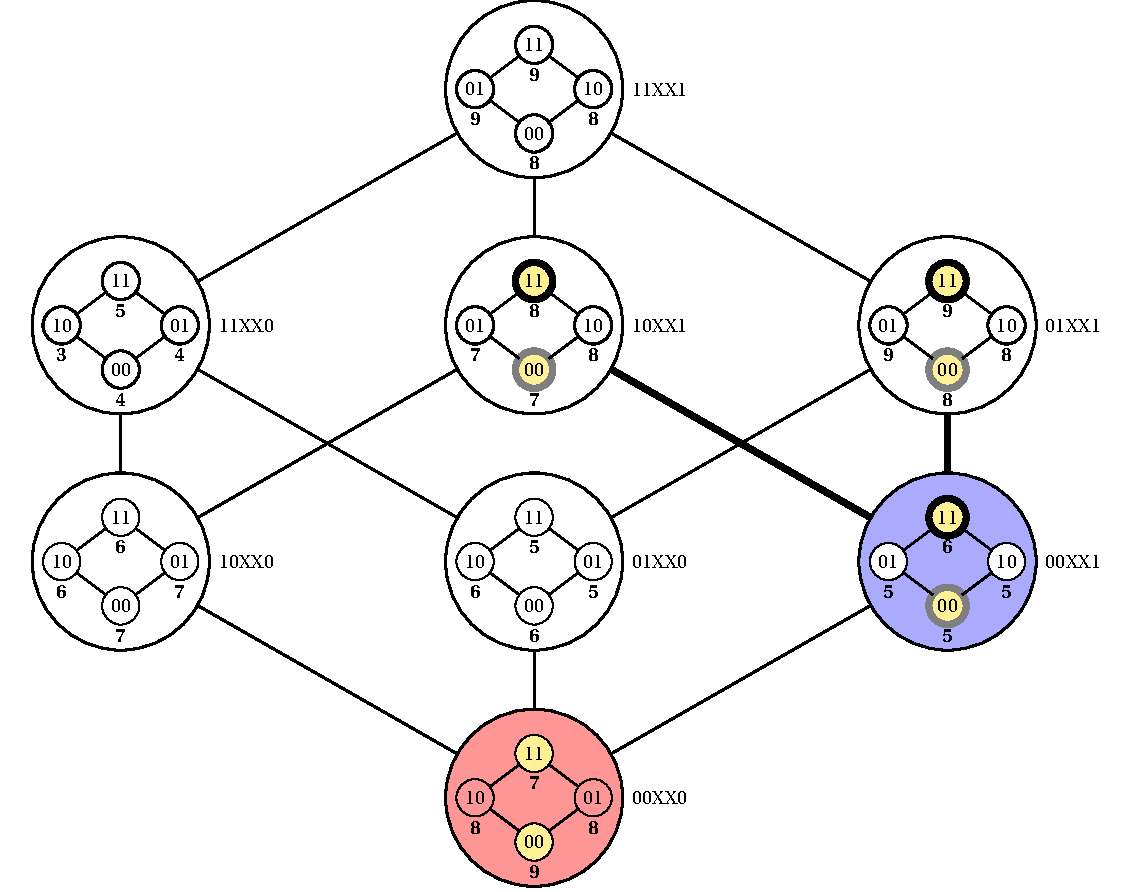
\includegraphics[clip=true, width=0.4\textwidth]{pucs/sample_run/C.pdf}
    }
    \vspace{1em}\pause\\ 
    \subfigure {
        \label{fig:pucs:example:D}
        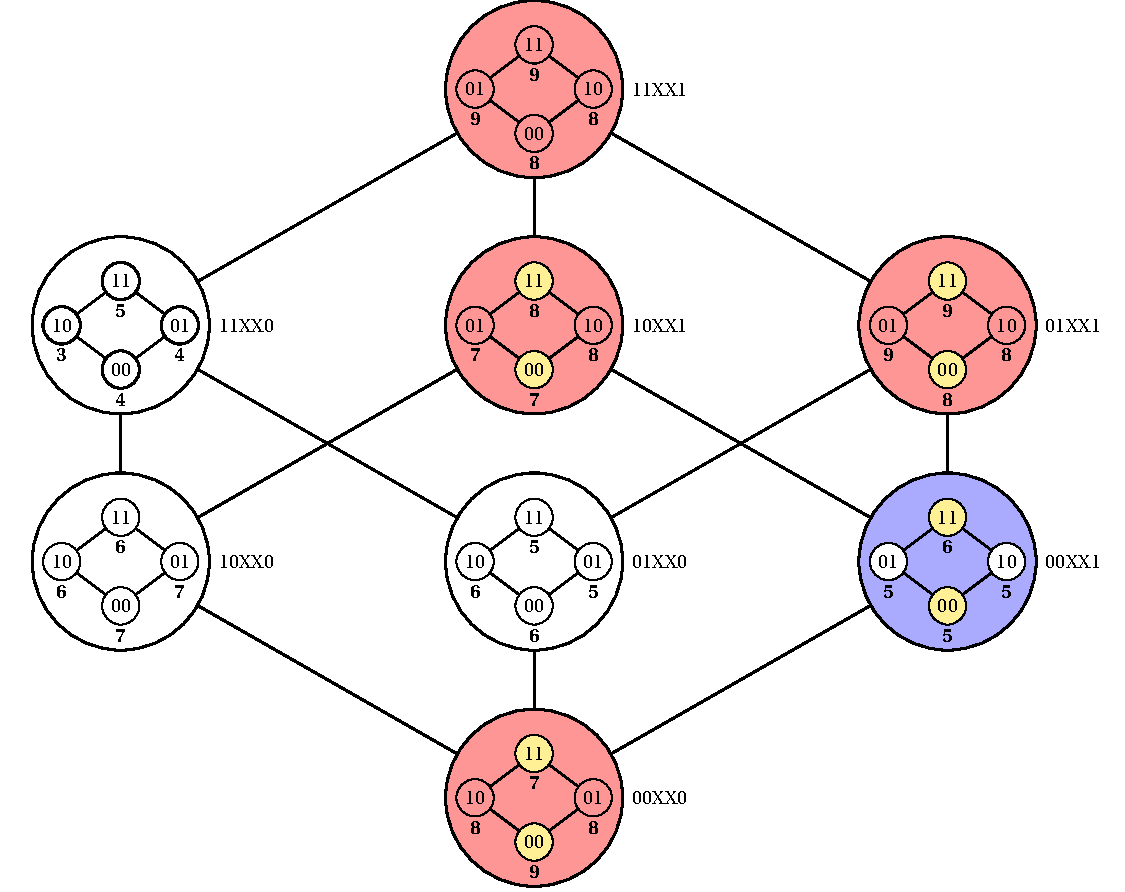
\includegraphics[ clip=true, width=0.4\textwidth]{pucs/sample_run/D.pdf}
    } \pause
    &
    \subfigure {
        \label{fig:pucs:example:E}
        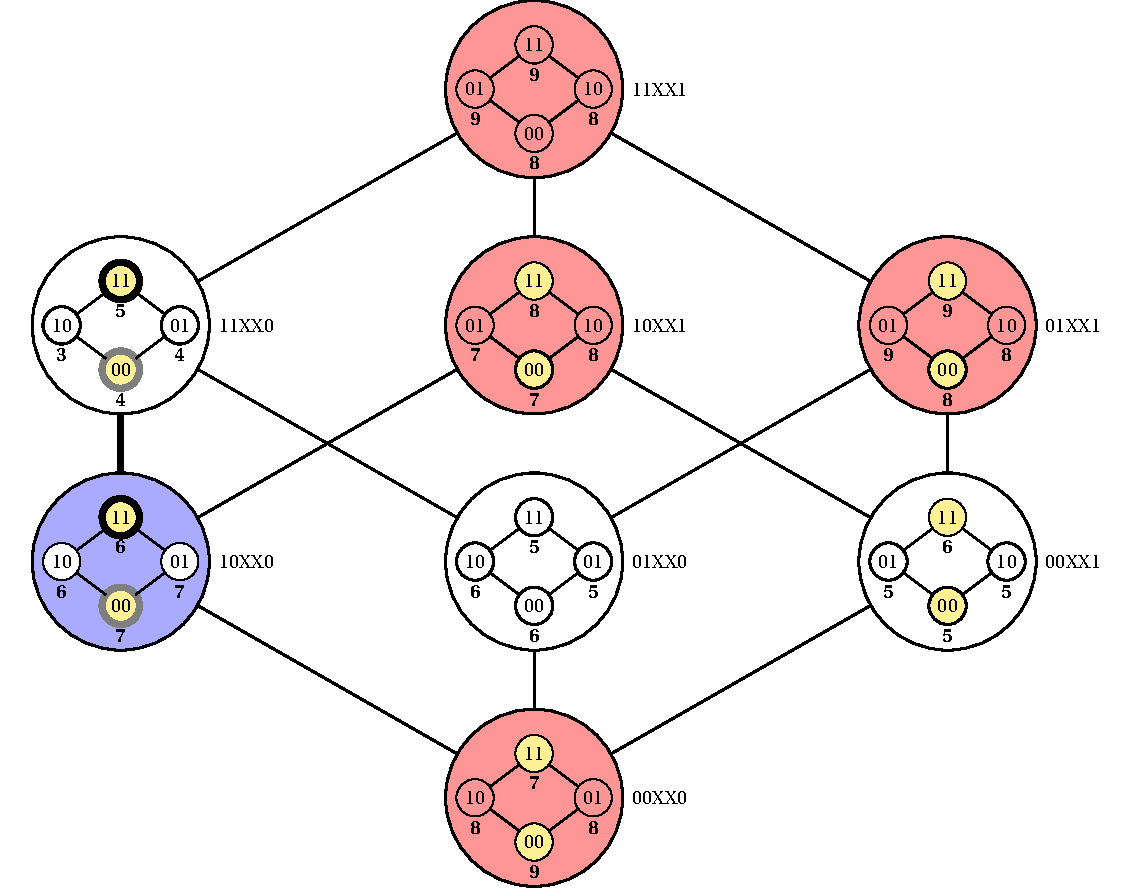
\includegraphics[clip=true, width=0.4\textwidth]{pucs/sample_run/E.pdf}
    }
    \end{tabular}   
    \end{center}
\end{figure}
\end{frame}


\begin{frame}{Simulação de execução}
\begin{figure}[]
    \begin{center}
    \begin{tabular}{l r}
    \centering
    \subfigure {
        \label{fig:pucs:example:F}
        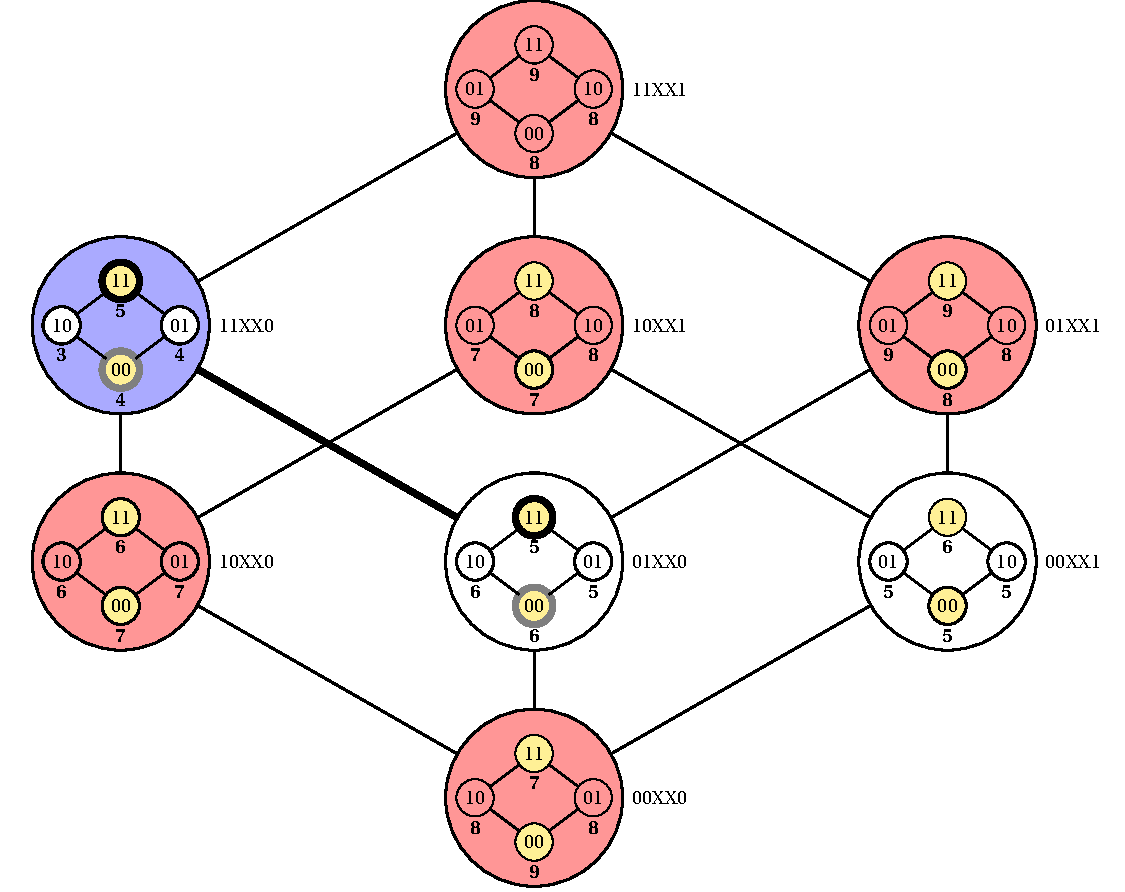
\includegraphics[ clip=true, width=0.4\textwidth]{pucs/sample_run/F.pdf}
    } \pause
    &
    \subfigure {
        \label{fig:pucs:example:G}
        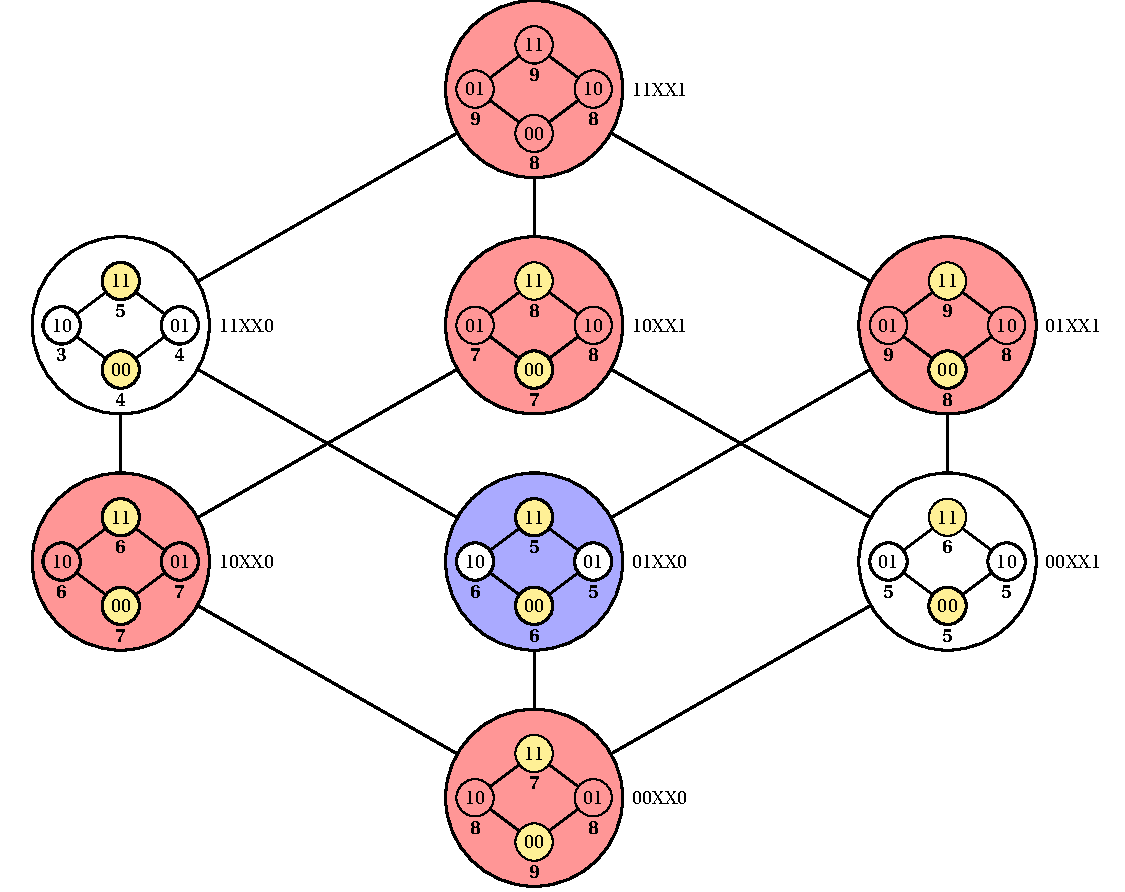
\includegraphics[clip=true, width=0.4\textwidth]{pucs/sample_run/G.pdf}
    }
    \vspace{1em}\pause\\
    \subfigure {
        \label{fig:pucs:example:H}
        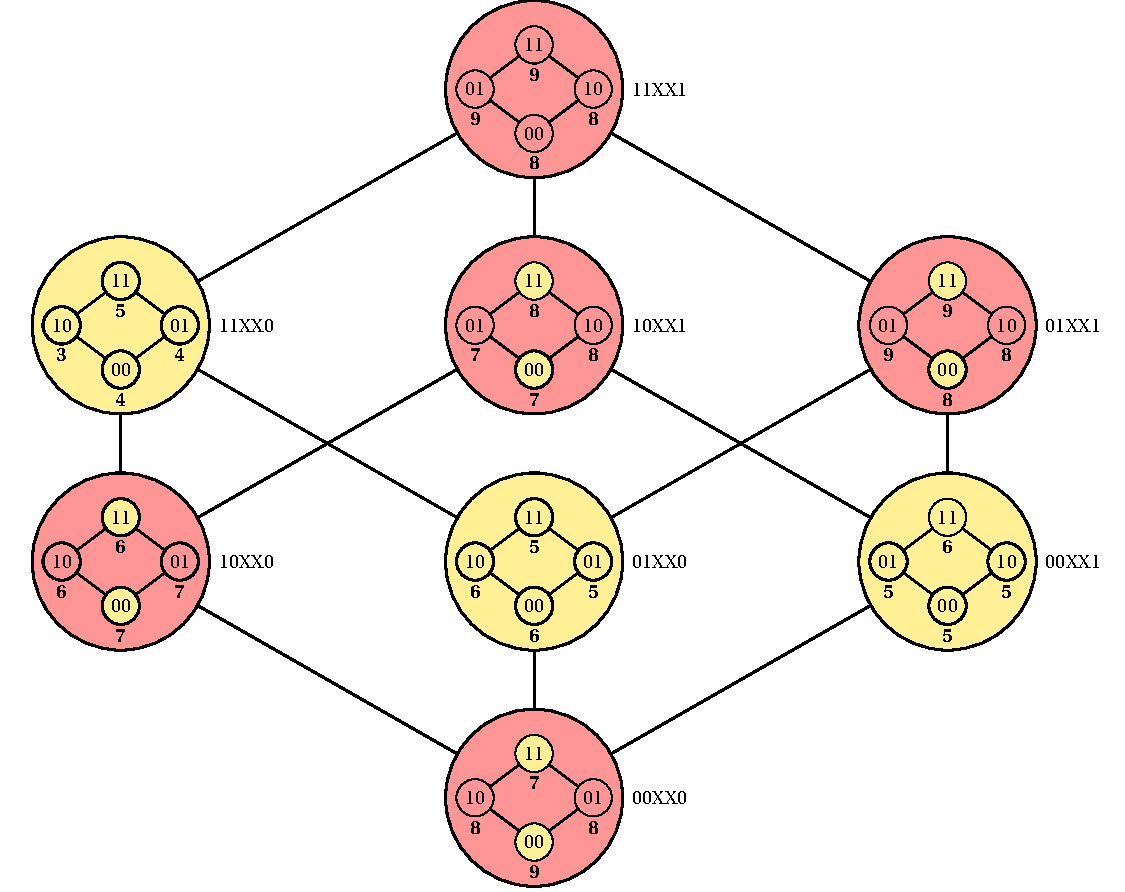
\includegraphics[ clip=true, width=0.4\textwidth]{pucs/sample_run/H.pdf}
    } \pause
    &
    \subfigure {
        \label{fig:pucs:example:I}
        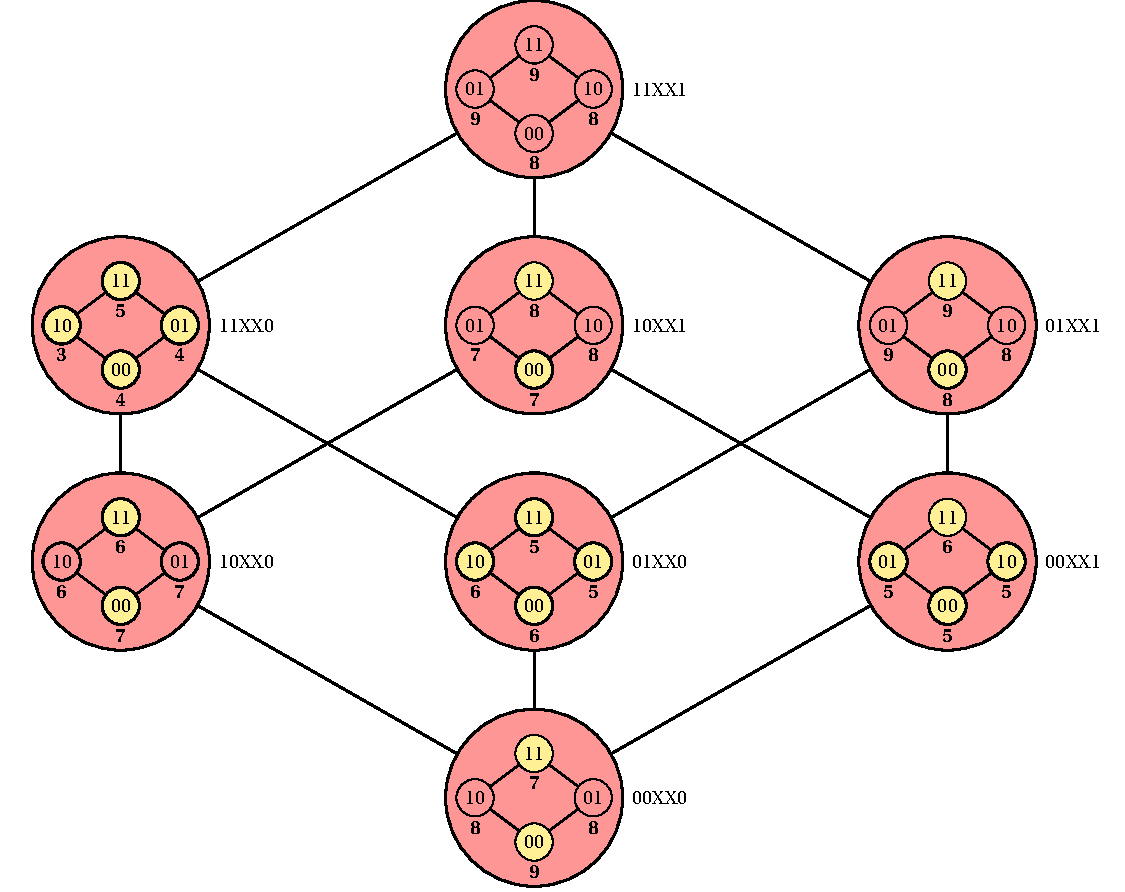
\includegraphics[clip=true, width=0.4\textwidth]{pucs/sample_run/I.pdf}
    }
    \end{tabular}   
    \end{center}
\end{figure}
\end{frame}

\begin{frame}{Parâmetros de funcionamento}
    O \algname{PUCS} tem parâmetros que controlam seu funcionamento:
    \pause
    \begin{itemize}
        \item{\alert{$p$} controla a quantidade de variáveis fixas;} \pause
        \item{\alert{$l$} controla a quantidade de chamadas recursivas do algoritmo;} \pause
        \item{um \alert{algoritmo base} que deve resolver as partes.}
    \end{itemize}
\end{frame}

\begin{frame}{Parâmetros de funcionamento}
    Os parâmetros $p$ e $l$ influenciam no tempo de execução do 
    algoritmo.
    \pause
    \begin{figure}
        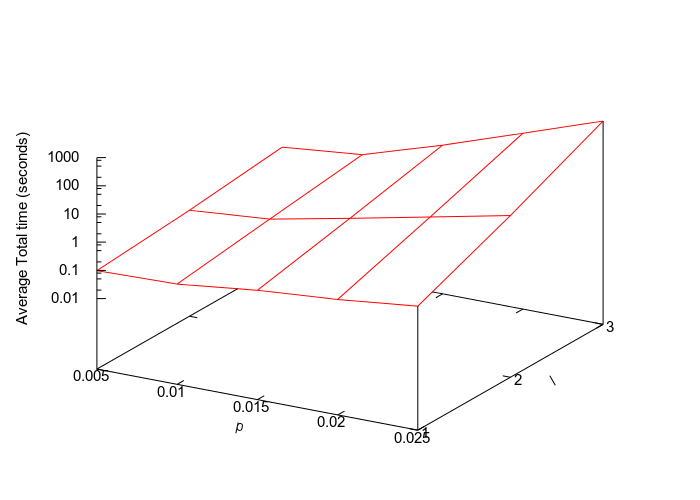
\includegraphics[clip=true, width=.6\textwidth]{pucs/parameters/n200-20-3_time.png}
    \end{figure}
    Quanto maior o valor dos parâmetros, maior o tempo de execução.
\end{frame}

\begin{frame}{Parâmetros de funcionamento}
    Quando o algoritmo base utilizado é ótimo, então o \algname{PUCS}
    também é ótimo.
    \vspace{1em}\pause

    Caso contrário, o \algname{PUCS} torna-se um heurística em que os
    parâmetros $p$ e $l$ influenciam na qualidade da solução.
    
    \begin{figure}
        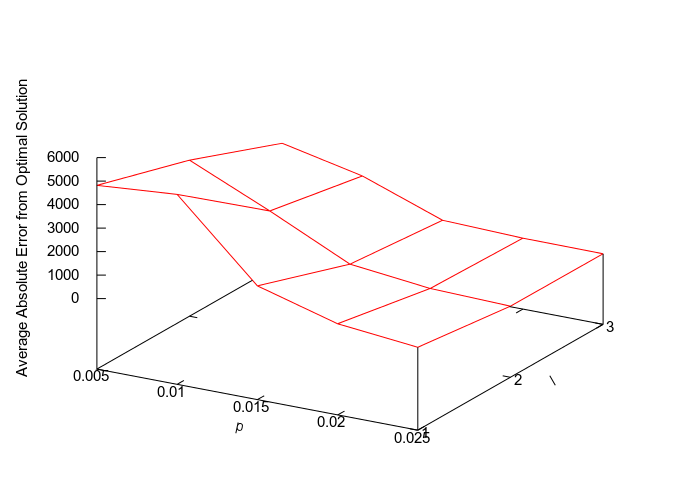
\includegraphics[clip=true, width=.6\textwidth]{pucs/parameters/n200-20-3_error.png}
    \end{figure}
\end{frame}

\begin{frame}{Resultados do \algname{PUCS}}
    Em instâncias pequenas, usamos parâmetros que deixam o algoritmo 
    ótimo.
    \begin{table}
    \resizebox{\columnwidth}{!}{
    \begin{tabular}{cc c cccc}
    \toprule
    \multicolumn{2}{c}{Instance} & \phantom{} & \multicolumn{4}{c}{Total time (sec)} \\
    \cline{1-2}\cline{4-7}\\
    $|S|$ & $2^{|S|}$ && \algname{UBB} & \algname{PFS} & \algname{UBB-PFS} & \algname{PUCS} \\
    % 10 &    1024 &&  0.006 $\pm$ 0.001 & 0.011 $\pm$ 0.002 & 0.022 $\pm$ 0.004 & 0.039 $\pm$ 0.019 \\
    % 11 &    2048 &&  0.007 $\pm$ 0.002 & 0.017 $\pm$ 0.004 & 0.026 $\pm$ 0.005 & 0.045 $\pm$ 0.022 \\
    % 12 &    4096 &&  0.009 $\pm$ 0.003 & 0.029 $\pm$ 0.009 & 0.033 $\pm$ 0.008 & 0.048 $\pm$ 0.024 \\
    % 13 &    8192 &&  0.013 $\pm$ 0.006 & 0.054 $\pm$ 0.016 & 0.047 $\pm$ 0.014 & 0.053 $\pm$ 0.021 \\
    % 14 &   16384 &&  0.026 $\pm$ 0.012 & 0.103 $\pm$ 0.035 & 0.074 $\pm$ 0.017 & 0.057 $\pm$ 0.024 \\
    % 15 &   32768 &&  0.048 $\pm$ 0.027 & 0.195 $\pm$ 0.080 & 0.116 $\pm$ 0.044 & 0.056 $\pm$ 0.025 \\
    % 16 &   65536 &&  0.097 $\pm$ 0.055 & 0.354 $\pm$ 0.176 & 0.198 $\pm$ 0.089 & 0.090 $\pm$ 0.080 \\
    % 17 &  131072 &&  0.142 $\pm$ 0.120 & 0.676 $\pm$ 0.375 & 0.350 $\pm$ 0.200 & 0.255 $\pm$ 0.276 \\
    18 &  262144 &&  \textbf{0.319 $\pm$ 0.228} & 1.512 $\pm$ 0.764 & 0.751 $\pm$ 0.338 & 0.680 $\pm$ 0.592 \\
    19 &  524288 &&  \textbf{0.684 $\pm$ 0.464} & 2.875 $\pm$ 1.554 & 1.387 $\pm$ 0.707 & 1.492 $\pm$ 1.323 \\
    20 & 1048576 &&  \textbf{1.249 $\pm$ 0.975} & 5.295 $\pm$ 3.509 & 2.594 $\pm$ 1.569 & 2.701 $\pm$ 2.908 \\
    21 & 2097152 &&  \textbf{2.671 $\pm$ 1.948} & 11.136 $\pm$ 6.947 & 5.460 $\pm$ 3.392 & 6.118 $\pm$ 5.961 \\
    22 & 4194304 &&  \textbf{5.420 $\pm$ 4.202} & 19.825 $\pm$ 14.519 & 9.709 $\pm$ 7.319 & 11.729 $\pm$ 11.613 \\
    \bottomrule
    \end{tabular}
    }
    \end{table}
\end{frame}


\begin{frame}{Resultados do \algname{PUCS}}
\begin{table}
\centering
\footnotesize
\resizebox{\columnwidth}{!}{%
\begin{tabular}{cc c cccc}
\toprule
\multicolumn{2}{c}{Instance} & \phantom{} & \multicolumn{4}{c}{\# Calls of cost function} \\
\cline{1-2}\cline{4-7}\\
$|S|$ & $2^{|S|}$ && \algname{UBB} & \algname{PFS} & \algname{UBB-PFS} & \algname{PUCS} \\
 % 1 &       2 && 2.0 $\pm$  0.0 &  2.0 $\pm$  0.0 &  2.0 $\pm$  0.0 &  5.0 $\pm$  0.0 \\
 % 2 &       4 && 3.8 $\pm$  0.4 &  3.9 $\pm$  0.2 &  3.8 $\pm$  0.4 &  7.4 $\pm$  0.9 \\
 % 3 &       8 && 6.9 $\pm$  1.3 &  7.7 $\pm$  0.5 &  6.9 $\pm$  1.3 & 15.0 $\pm$  3.2 \\
 % 4 &      16 && 13.1 $\pm$  3.5 & 13.1 $\pm$  2.9 & 13.1 $\pm$  3.5 & 28.6 $\pm$  8.1 \\
 % 5 &      32 && 25.0 $\pm$  8.2 & 25.4 $\pm$  5.1 & 24.4 $\pm$  7.5 & 50.3 $\pm$ 14.4 \\
 % 6 &      64 && 50.7 $\pm$ 16.7 & 49.6 $\pm$ 13.9 & 49.3 $\pm$ 14.4 & 97.8 $\pm$ 32.9 \\
 % 7 &     128 && 101.6 $\pm$ 34.2 & 80.2 $\pm$ 29.3 & 95.1 $\pm$ 24.9 & 167.4 $\pm$ 57.6 \\
 % 8 &     256 && 166.2 $\pm$ 89.6 & 173.0 $\pm$ 33.9 & 162.7 $\pm$ 69.7 & 274.1 $\pm$ 136.8 \\
 % 9 &     512 && 356.2 $\pm$ 193.1 & 313.0 $\pm$ 91.9 & 323.1 $\pm$ 126.6 & 472.8 $\pm$ 285.4 \\
% 10 &    1024 && 668.2 $\pm$ 359.2 & 614.2 $\pm$ 162.7 & 630.3 $\pm$ 235.9 & 753.6 $\pm$ 493.6 \\
% 11 &    2048 && 1171.5 $\pm$ 742.5 & 1139.2 $\pm$ 354.0 & 1174.8 $\pm$ 499.3 & 1305.0 $\pm$ 881.8 \\
% 12 &    4096 && 2611.6 $\pm$ 1528.5 & 2137.1 $\pm$ 793.3 & 2271.2 $\pm$ 894.1 & 2370.5 $\pm$ 1615.7 \\
% 13 &    8192 && 4583.2 $\pm$ 2910.2 & 4218.9 $\pm$ 1306.7 & 4308.7 $\pm$ 1732.2 & 4780.0 $\pm$ 2797.7 \\
% 14 &   16384 && 10781.4 $\pm$ 5565.5 & 8211.1 $\pm$ 3054.5 & 9050.4 $\pm$ 2638.1 & 7050.8 $\pm$ 4755.7 \\
% 15 &   32768 && 20891.9 $\pm$ 12757.0 & 15134.0 $\pm$ 6528.5 & 15900.7 $\pm$ 6927.4 & 14080.1 $\pm$ 11373.1 \\
16 &   65536 && 43529.6 $\pm$ 25318.9 & 26447.0 $\pm$ 13446.1 & \textbf{28783.6 $\pm$ 12934.2} & 26001.3 $\pm$ 21699.6 \\
17 &  131072 && 65301.0 $\pm$ 56215.8 & 49694.5 $\pm$ 27621.8 & \textbf{51032.5 $\pm$ 29984.3} & 50145.2 $\pm$ 46799.0 \\
18 &  262144 && 145594.5 $\pm$ 103597.8 & 105603.1 $\pm$ 52652.2 & \textbf{110538.0 $\pm$ 51589.7} & 111296.6 $\pm$ 84922.4 \\
19 &  524288 && 313096.0 $\pm$ 209913.1 & 194572.5 $\pm$ 104802.3 & \textbf{204604.5 $\pm$ 100305.4} & 233717.7 $\pm$ 186182.0 \\
20 & 1048576 && 578319.0 $\pm$ 445912.2 & 340052.5 $\pm$ 221271.6 & \textbf{362007.0 $\pm$ 207411.2} & 387082.0 $\pm$ 389417.4 \\
% 21 & 2097152 && 1208939.1 $\pm$ 867260.3 & 699906.1 $\pm$ 437209.1 & 726193.9 $\pm$ 420497.8 & 854293.9 $\pm$ 779635.6 \\
% 22 & 4194304 && 2375634.9 $\pm$ 1826536.5 & 1195439.1 $\pm$ 881956.5 & 1253704.3 $\pm$ 847533.7 & 1640138.3 $\pm$ 1547703.6 \\
\bottomrule
\end{tabular}
}
\end{table}
\end{frame}

\begin{frame}{Resultados do \algname{PUCS}}
Em experimentos sub-ótimos, comparamos o \algname{PUCS} com as 
heurísticas \algname{Sequential Forward Floating Search} 
(\algname{SFFS}) e \algname{Best-First Search} (\algname{BFS}).
\begin{figure}[!ht]
\begin{center}
\begin{tabular}{l r}
\centering
\subfigure {
    \label{fig:pucs:big:time}
    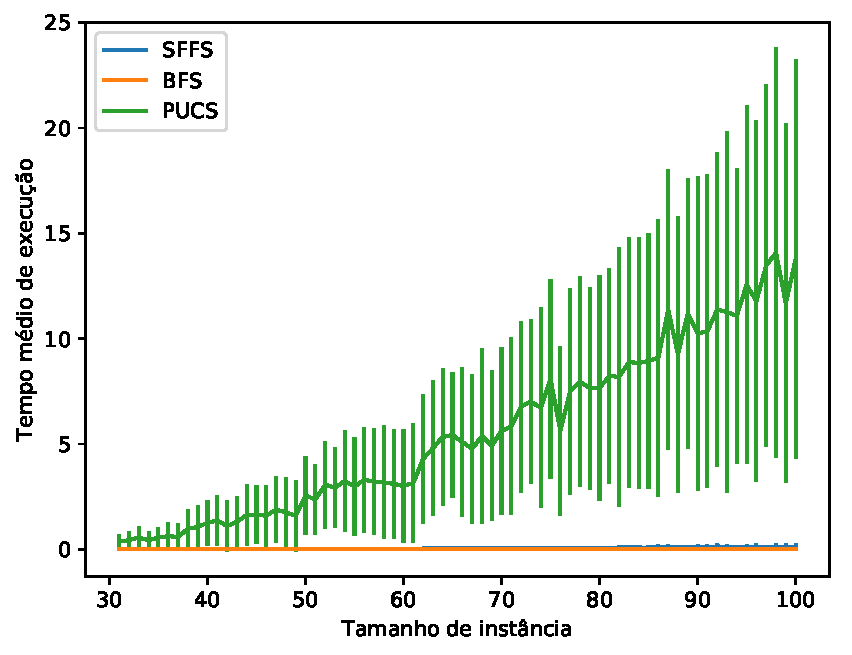
\includegraphics[clip=true, width=0.45\textwidth]{pucs/experiments/time_sffs_bfs_pucs.pdf}
}
&
\subfigure {
    \label{fig:pucs:big:correctness}
    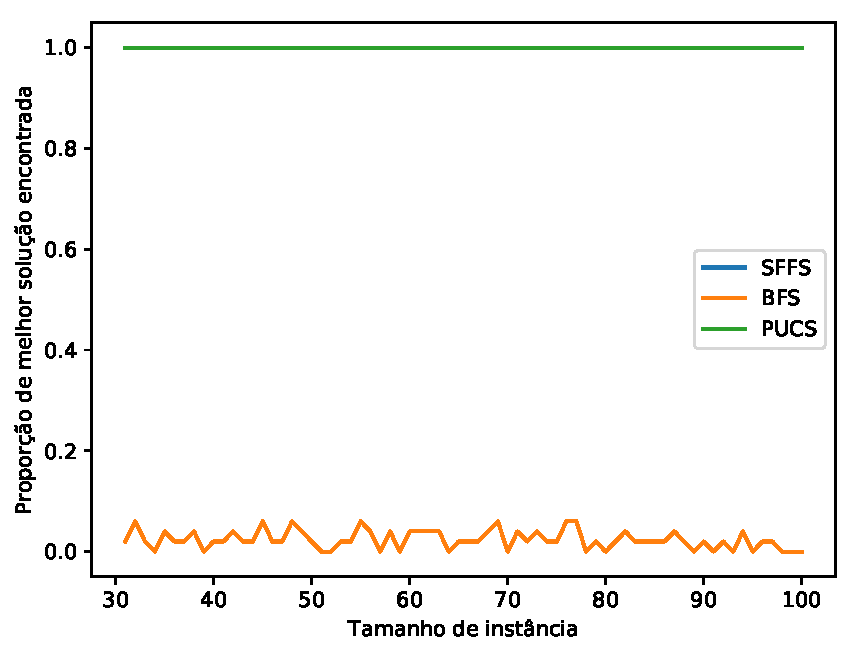
\includegraphics[clip=true, width=0.45\textwidth]{pucs/experiments/correctness_sffs_bfs_pucs.pdf}
}
\end{tabular}   
\end{center}
\end{figure}
\end{frame}

\section{Aplicações instâncias reais}

\begin{frame}{Seleção de características em seleção de modelos}
    Aplicamos seleção de características na construção de modelos
    de aprendizado para conjuntos de dados do UCI Machine Learning
    Repository.
\end{frame}

\begin{frame}{Modelos de aprendizado}
    Os modelos que utilizamos para o treinamento e classificação
    são do tipo Support Vector Machine.
    \begin{figure}
        \centering
        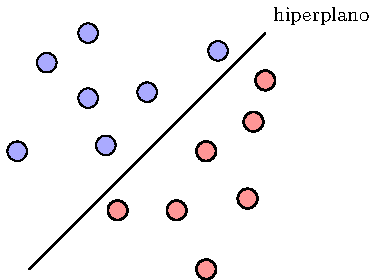
\includegraphics[clip=true, width=.5\textwidth]{svm/svm.pdf}
    \end{figure}
\end{frame}

\begin{frame}{Conjuntos de dados testados}
Fizemos o treinamento e validação de modelos de aprendizado nos 
seguintes conjuntos de dados: \pause
    \begin{itemize}
        \item{Iris} \pause
        \item{Wine} \pause
        \item{Thoracic Surgery} \pause
        \item{Zoo} \pause
        \item{Breast Cancer} \pause
        \item{Lung Cancer} \pause
        \item{Promoters} \pause
    \end{itemize}
\end{frame}


\begin{frame}{Validação cruzada}
Para avaliar a seleção de características fizemos a validação cruzada
de modelos com todas características e a de modelos apenas com 
características selecionadas.
\end{frame}

\begin{frame}{Resultados}
    O número de características selecionadas é, de fato, menor do que
    o conjunto inteiro.\pause
    \begin{figure}
        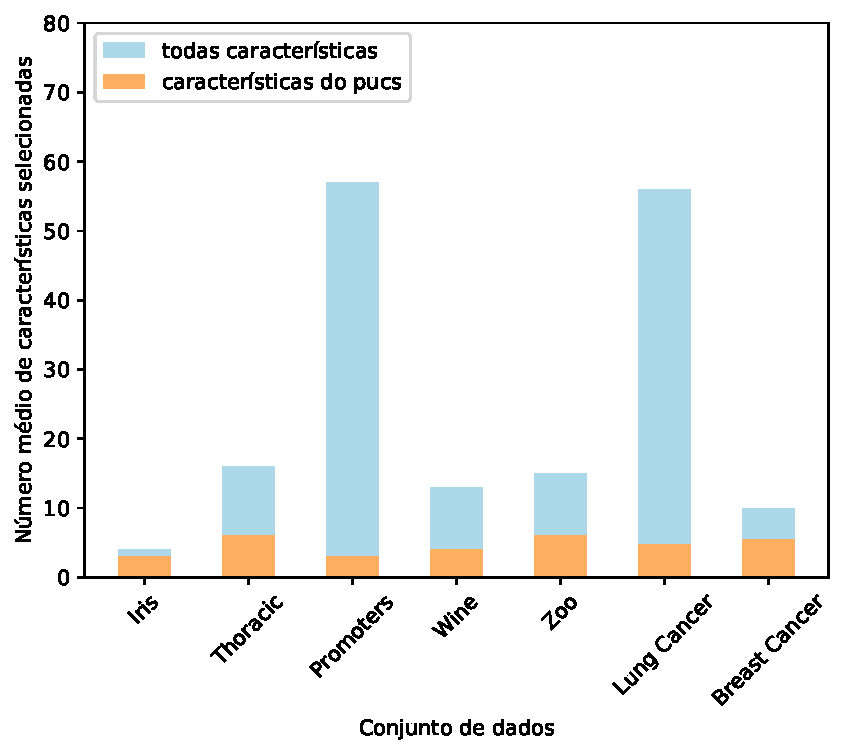
\includegraphics[clip=true, width=0.6\textwidth]{uci/avg_features.pdf}
    \end{figure}
\end{frame}

\begin{frame}{Resultados}
    Além disso, a qualidade dos modelos não é afetada. \pause
    \begin{figure}
        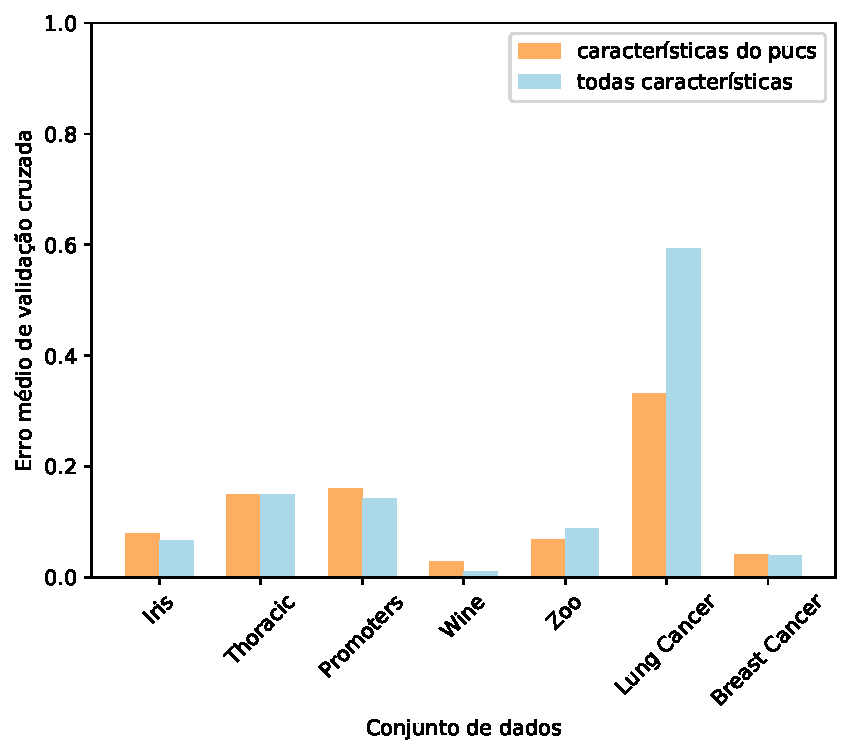
\includegraphics[clip=true, width=0.6\textwidth]{uci/svm_error.pdf}
    \end{figure}
\end{frame}

\section{Revisão}
\begin{frame}{Revisão dos resultados deste trabalho}
Ao longo deste trabalho apresentamos \pause
    \begin{itemize}
        \item{Modificações no \algname{PFS}.}
        \begin{itemize}
            \item{Escolha de raízes.}
            \item{Estrutura de dados para armazenamento de raízes.}
        \end{itemize} \pause
        \item{Uma paralelização do \algname{PFS}.} \pause
        \item{O algoritmo \algname{UBB-PFS}.} \pause
        \item{O algoritmo \algname{PUCS}.} \pause
        \item{Testes com instâncias reais.} \pause
    \end{itemize}
\end{frame}
\end{document}


